%%%% Proceedings format for most of ACM conferences (with the exceptions listed below) and all ICPS volumes.
\documentclass[manuscript, review=True]{acmart}
\settopmatter{printacmref=false} % Removes citation information below abstract
\renewcommand\footnotetextcopyrightpermission[1]{} % removes footnote with conference information in first column
\pagestyle{plain} % removes running headers

\usepackage[utf8]{inputenc}
\usepackage[english]{babel}
\usepackage{amsmath}
\usepackage{url}
\usepackage{subfig}
\usepackage{float}
\usepackage{graphicx}
\usepackage{setspace}
%\setlength{\parskip}{1em}
\pagenumbering{arabic}
\pagestyle{fancy}
\usepackage{pbox}
% excel2latex
\usepackage{multirow}
\usepackage{xcolor}
\usepackage{colortbl}
\usepackage{rotating}
\usepackage{booktabs,arydshln}

\makeatletter
\def\adl@drawiv#1#2#3{%
        \hskip.5\tabcolsep
        \xleaders#3{#2.5\@tempdimb #1{1}#2.5\@tempdimb}%
                #2\z@ plus1fil minus1fil\relax
        \hskip.5\tabcolsep}
\newcommand{\cdashlinelr}[1]{%
  \noalign{\vskip\aboverulesep
           \global\let\@dashdrawstore\adl@draw
           \global\let\adl@draw\adl@drawiv}
  \cdashline{#1}
  \noalign{\global\let\adl@draw\@dashdrawstore
           \vskip\belowrulesep}}
\makeatother

%define code command
\definecolor{light-gray}{gray}{0.95}
\newcommand{\code}[1]{\colorbox{light-gray}{\texttt{#1}}}

% Copyright
\setcopyright{none}

% DOI
% \acmDOI{10.475/123_4}

% ISBN
% \acmISBN{123-4567-24-567/08/06}

%Conference
\acmYear{2017}

% \acmArticle{4}
% \acmPrice{15.00}

% These commands are optional

\begin{document}
\title{Accurate, scalable microbiome quantification with shallow shotgun sequencing}

\author{Benjamin Hillmann}
\orcid{0000-0003-4276-1329}
\affiliation{%
  \institution{University of Minnesota}
  \streetaddress{100 Church Street SE}
  \city{Minneapolis} 
  \state{Minnesota} 
  \postcode{55455}
}
\email{hillmannben@gmail.com}


% The default list of authors is too long for headers.
\renewcommand{\shortauthors}{Benjamin Hillmann}

\begin{abstract}
Despite the association of microbial communities with many aspects of human, environmental, plant, and animal health, there exists no cost-efficient method for precisely characterizing the species and genes present in a microbial community. Current methods that use affordable amplicon sequencing techniques cannot resolve taxonomy past the genus level and only can classify clades whose genome has the marker gene. While deep whole-genome shotgun (WGS) is able to solve these problems, the technique is prohibitively expensive for large-scale studies. To address these issues, we propose a novel computational pipeline SHOGUN using shallow whole-genome shotgun (shallow shotgun) sequencing that recovers accurate taxonomic profiles of human microbiomes. We show that by sequencing at fraction of the cost and depth of WGS surveys, we can provide nearly the same measured species-level taxonomic profile. We demonstrate the shallow shotgun results on multiple real biological datasets and simulated communities. The pipeline SHOGUN relies on whole-genome reference databases, and is therefore most useful for well-characterized environments such as the human microbiomes in the gut, skin or oral cavity. Thus, SHOGUN allows researchers to obtain near-WGS data quality at only slightly higher cost than amplicon sequencing, enabling a fundamental shift toward higher precision in human microbiome research.
\end{abstract}

%
% The code below should be generated by the tool at
% http://dl.acm.org/ccs.cfm
% Please copy and paste the code instead of the example below. 
%
% \begin{CCSXML}
% <ccs2012>
% <concept>
% <concept_id>10010405.10010444.10010087.10010934</concept_id>
% <concept_desc>Applied computing~Computational genomics</concept_desc>
% <concept_significance>500</concept_significance>
% </concept>
% </ccs2012>
% \end{CCSXML}

% \ccsdesc[500]{Applied computing~Computational genomics}


% \keywords{ACM proceedings}


\maketitle

% \listoffigures
% \listoftables

\section{Introduction}

Microbial community structure is associated with many aspects of human, plant, animal, and environmental health; despite this, there are currently no affordable methods to characterize what species and genes are present in a given community \cite{prifti_new_2013}. Unfortunately, most of the microbes in these communities cannot be cultured, so to observe the biological contents of these communities we must quantify their taxonomic profiles through sequencing the microbes DNA. This has led to a dramatic influx of large metagenomic datasets and a surge in the demand for scientists to precisely describe the species within these communities to determine which organisms are beneficial and which are detrimental for different environments and applications.

Microbiome DNA analysis is typically performed in one of two ways: using amplicon-based (16S) or whole-genome shotgun-based (WGS) sequencing methods. Amplicon based techniques typically amplify a highly variable region of the 16S ribosomal RNA gene, although other genes may be targeted in particular cases, such as for fungal microbiome sequencing. Amplicon sequencing is affordable, but often cannot distinguish between species due to sequence similarities, and does not allow high-accuracy prediction of the functional repertoire. Because amplicon methods rely on DNA primers to amplify the region of interest, they are also subject to high levels of bias and can fail to capture organisms whose DNA sequence does not match the primers. As an alternative, WGS sequencing sequences randomly selected fragments of all DNA present in a microbiome. WGS directly measures the functional repertoire of the microbiome by capturing a snapshot of the total metagenomic content and allows strain-level characterization of microbiomes by mapping reads to the unique markers of strain reference genomes. WGS, however, is typically ten times more expensive than amplicon sequencing due to its use of costly library preparation protocols and and the additional costs of very deep sequencing. This forces researchers to choose between affordability with amplicon methods, and accuracy with WGS.

A major concern for the use of any taxonomic quantification profile is having the ability to identify and quantify distinct taxonomic clades from within a complex community. If a strain is able to be grown in a monoculture or isolated, deep coverage of its genome allows precise assembly and annotation of its strain-specific polymorphisms (SNP), functional genes and other higher level functional modules. The assembled genomes and annotations are then placed in a database \cite{tatusova_refseq_2014}, and can be utilized as a reference genome for taxonomic profiling. In mixed microbial communities, such as the human gut microbiome, a WGS survey has been shown to be effective at recovering the species-to-strain specific taxonomic profile of the community. However, as previously mentioned, WGS are prohibitively expensive due to the high sequencing depth required for coverage of genome assembly, traditional low multiplexing of samples submitted to be sequenced, and SNP detection in individual strains. The goal of microbiome surveys is not always for the assembly of individual strains, but often is looking for differential microbial communities between disease states. Due to this goal, the exploration of accurate species level taxonomic profiles at varying shotgun sequencing depths should be explored to reduce costs of research with different objectives.

Development of robust yet affordable methods for accurate microbial profiling is a major priority for the microbiome research field. The critical barriers to quantifying microbiomes at the species level that are affordable, accurate and reproducible. Overcoming the shortcomings of amplicon and shotgun techniques presents major challenges in the field of metagenomics, and prevents scientists from performing highly precise, large-scale studies. After microbial communities have been sequenced, it is the objective of the researcher to utilize informatics methods to correlate the taxonomic and functional profiles of a sample to a trait of interest. However, these methods operate under the assumption that the underlying taxonomic and functional profiling are accurate. If methods are developed to more accurately identify the profiles of a community, the increased precision will cascade down every step along the metagenomics pipeline. With more precise profiles, the informatics methods will have more power to test hypotheses and better ability detect the causal role these communities play. Accurate cost- and time-effective taxonomic quantification of environmental samples is essential. Given the weaknesses of the aforementioned techniques, we propose novel highly data-efficient methods for species- and strain-level resolution taxonomic profiles in low-depth shotgun metagenomic datasets (shallow shotgun).

Here we describe a novel approach using shallow shotgun sequencing, combined with our proposed shallow shotgun (SHOGUN) analysis pipeline \cite{benjamin_hillmann_knights-lab/shogun:_2017}, as an alternative to WGS sequencing. We show through analysis of several biological data sets and through simulated data that SHOGUN provides nearly the same accuracy at the species and functional level as deep WGS sequencing, but at a small fraction of the cost, with materials and DNA sequencing with comparable cost to amplicon sequencing. Thus, we expect that SHOGUN will allow researchers to switch immediately from marker gene sequencing to shallow shotgun sequencing for little additional cost and large accuracy payoff.

\section{Materials and Methods}

A typical protocol for going from next-generation sequencing (NGS) reads of a mixed community to a taxonomic profile counts per clade is described in \textit{Figure ~\ref{fig:taxonomic_profiler}}. Depending on the taxonomic profile tool used, the steps in the protocol can vary widely. We chose to evaluate tools against our taxonomic profiler SHOGUN \cite{benjamin_hillmann_knights-lab/shogun:_2017} pipeline based on their ease of use and documentation, availability as an open-source tool, the ability to create a user defined database, summarize a taxonomy profile at the species level, and the ability to scale to large datasets with multiple threads per process. As a result of these requirements, we decided to evaluate the effectiveness of the tools Centrifuge \cite{kim_centrifuge:_2016} and Kraken \cite{wood_kraken:_2014}.

\subsection{SHOGUN Pipeline for Metagenomic Relative Abundance Estimation}

The SHOGUN pipeline for metaganomic taxonomic profiling is described in \textit{Figure ~\ref{fig:shogun_schematic}}. The taxonomic profiling algorithm with SHOGUN is broken up into three major steps: alignment, taxonomic read assignment, and rank-specific relative abundance estimation. There are three alignment tools, Bowtie2 \cite{langmead_fast_2012}, BURST \cite{gabriel_al-ghalith_knights-lab/burst:_2017}, and UTree \cite{gabriel_al-ghalith_knights-lab/utree:_2017}, implemented for use within SHOGUN, and each of which was tested to find their specific advantages and disadvantageous.

\subsubsection{Bowtie2 Burrows-Wheeler Alignment}

The alignment tool Bowtie2 \cite{langmead_fast_2012} is a fast gapped read alignment tool utilizing the Burrows-Wheeler transform. We modified the \code{bowtie2} command from its default settings so that matches to ambiguous bases are penalized, sequential gaps are weighted differently than single gaps, and that up to 32 valid alignments above the specified percent identification are reported. To save space, the header and unaligned sequences were set to be suppressed. The command line to target these behaviors \cite{al-ghalith_ninja-ops:_2016}:

\begin{center}
	\code{--no-unal --np 1 --mp "1,1" --rdg "0,1" --rfg', '"0,1" --score-min "L,0,-0.02" -k 32 --no-hd}
\end{center}

The percent identification threshold is set by the \code{--score-min} function  as \%ID/100-1. In this case, to match above 98\% percent identification (same as the BURST aligner) the parameter \code{--score-min} is set to $100-1=-0.02$. We do not recommend changing these settings to retain compatibility for downstream SHOGUN analysis.

As previously specified, for each query sequence there can be up to 32 valid alignments. In order to assign a taxonomy to the query sequence given the valid alignments, we report the last common ancestor of all the taxonomic lineages of the valid alignments.

\subsubsection{BURST Optimal Alignment}

BURST is an exhaustive optimal aligner leveraging dynamic programming in rapidly identifying and computing all valid alignments above a specified BLAST identification cutoff and or all best ties. It has to two primary reporting modes utilized in SHOGUN.


\begin{itemize}

 \item \textbf{Capitalist} Capitalist enumerates all tied best hits above the user specified identity cutoff. The goal of capitalist mode is to return the minimal set of references that best explain all queries. It meets these requirements by translating the problem to finding the minimum set of query nodes in a bipartite graph such that each query is connected to a single reference. In the bipartite graph, one partite of nodes is queries and one partite of nodes is reference genomes. The edges in the graph are the valid best hits. Finding the minimum set of references is found by greedily pruning legal edges, until each query retains only a single edge. The order of the edges for pruning is set by a priority queue. The edge priority in the queue is sorted in descending order of highest degree reference nodes. Every edge is placed into the priority queue and enumerated. For every edge in the priority queue, the edge is pruned if the degree of the connected query is greater than one. If an edge is pruned, the priorities of each other edge of the respective query is updated in the priority queue with the new query degree. The pruning algorithm terminates once each query vertex is degree one. In the final report, the edge and corresponding alignment for each query is reported.

\item \textbf{Taxonomy} Taxonomy mode is similar to capitalist mode in that it enumerates all tied best hits above the user specified identity cutoff. It differs in that its goal is to return the most likely taxonomic annotation for a given query similar to the aufbau voting rounds of UTree. That is, for each query sequence, the set of valid alignments taxonomic annotation above the user specified threshold is enumerated. The first voting round begins at the highest rank, where each of the alignments for a given query vote for their respective taxonomic rank. A If a plurality of the unique taxonomic votes is determined to be above the user specified threshold, the default threshold being 75\%, all children of that taxonomic rank are used in the next round of voting. Voting rounds continue until a taxonomic lineage leaf is reached or the plurality supporting vote does not exceed the threshold. If a round of voting does not exceed the specified support threshold, the interpolation stops and the last rounds taxonomic lineage vote is returned for the query.

\end{itemize}

\subsubsection{UTree k-mer Classification}

The tool UTree is an alignment-free sequence analysis tool that maps short reads to reference genomes using a k-mer indexing scheme similar to that of CLARK \cite{ounit_higher_2015} and Kraken \cite{wood_kraken:_2014}. The purpose of UTree is to be light on computational resources will still being able to search query sequences up to 16 Megabase pairs in length against full sized reference genomes. It uses an efficient, unique k-mer indexing schemes of reference taxonomic ranks through the use of a prefix-forest and suffix binary tree. The database is built by stepping through each input reference sequence and determining whether each k letter window, known as a k-mer, is unique to that references taxonomic rank. When a k-mer is selected from the reference genome to be inserted into the database, it can be flagged as either unique or ambiguous to a specific taxonomic rank. In the case that the k-mer is unique to the lowest taxonomic rank, the k-mer is added to the suffix binary tree at the index retrieved from the prefix-forest location with the associated taxonomic metadata. In the case where the k-mer is not unique, the existing k-mer's taxonomic rank within the database is demoted to the common ancestor of the current reference and the existing taxonomy. If the common ancestor is the root, it is excluded from the database when searching. When searching a query sequence, all unambiguous k-mers in the query are searched for in the database. All k-mers that were found in the database are used to interpolate the taxonomic identity of the query in what is called 'aufbau' voting rounds. The first voting round starts at the highest taxonomic rank, in this case it would be kingdom. A vote is placed for a taxonomic lineage for each uniquely identified k-mer from the query sequence. If a plurality of the unique k-mer votes is determined to be above the user specified threshold, the default threshold being 75\%, all children of that taxonomic rank are used in the next round of voting. Voting rounds continue until a taxonomic lineage leaf is reached or the plurality supporting vote does not exceed the threshold. If a round of voting does not exceed the specified support threshold, the interpolation stops and the last rounds taxonomic lineage vote is returned for the query.

\subsubsection{Relative Abundance Estimation Through Redistribution}

The job of most taxonomic profilers is to assign a taxonomic classification to each query sequence from a metagenomic sample. However, in rank-flexible annotations, converting higher level taxonomic annotations, such as the rank family, to a lower rank annotation, such as the rank species, can produce erroneous results if you do not account for differences genetic diversity across the taxonomic tree. In order to resolve those challenges for rank-flexible classifiers, SHOGUN re-introduces the principle of Bayesian redistribution of reads in a similar fashion to the Bracken algorithm \cite{lu_bracken:_2017}. That is, at higher levels of the taxonomic tree are redistributed to lower levels according to each genomes uniqueness and length.

The major difference between the original Bracken algorithm and the redistribution algorithm for SHOGUN is how the uniqueness probabilities $U_i$ are calculated for each respective genome $i$ in the database. In Bracken, each genome in the database was sheared with a sliding window of size $r$ and step size of 1 creating $(L_i + r + 1)$ taxonomic annotations for each genome classified by Kraken \cite{wood_kraken:_2014}. We swap out the classification tool Kraken with the optimal alignment tool BURST. We set BURST to recover all alignments above a 98\% alignment identification using capitalist and increase the step size for the shearing of the genomes to 50. When capitalist resolves its hits, we assign the taxonomic annotation to be the last common ancestor of the genome that the sheared read was taken from and the genome that was classified. This holds the advantages that BURST can recover the locations of genome redundancy, higher precision in classification of reads, and the relative abundance re-estimation is provided through the tools used within SHOGUN to remain consistent.

\subsection{Materials}

\subsubsection{SHOGUN Database}

To validate the performance of taxonomic classification at varying sequencing depths, we selected a database that contained fully assembled genomes that were filtered to adequately cover all branches of the taxonomic tree of life as best as possible. The database of genomes for all analysis and tools in this paper was all complete, representative Archaea, Bacteria, Plasmid, Viroids and Virus genomes from the reference database RefSeq version number 82 (Rep82) as of May 8, 2017 \cite{tatusova_refseq_2014}. Explanations of the microbes present in this reference genome database are shown in \textit{Table ~\ref{tab:database_stats}}. The contaminate database was the human genome assembly obtained from the Genome Reference Consortium Human Build 38 (GRCh38) with no alternate scaffolds \cite{staff_introducing_2013}.

\subsubsection{Human Microbiome Project Shotgun Dataset}

We tested the ability to discriminate between human microbiomes source body sites at varying sequence depths. Quality controlled and contaminate filtered WGS samples were selected from the Human Microbiome Project \cite{consortium_structure_2012}. Up to 30 representative samples were selected from each body site if available (tongue dorsum; $n = 30$, stool; $n = 30$, supragingival plaque; $n = 30$; subgingival plaque; $n = 7$, right retroauricular crease; $n=14$, left retroauricular crease; $n = 9$).

The HMP sequence data were aligned against the Rep82 database using SHOGUN BURST capitalist mode at full depth, and redistribution to species level taxonomy. To account for experimental differences in sample sequencing depth, we normalized sample counts to the median sequencing depth \cite{mcmurdie_waste_2014}. Each full depth count sample vector was than re-sampled to specific depths (10, 100, 10 thousand, 100 thousand, 1 million, 10 million and a 100 million) by bootstrap sampling with replacement. Each count vector was subsampled to contain only taxonomies that existed in 33\% of all samples, with a detection limit of one read per million on average. Finally, the data were transformed using multiplicative replacement and centered log-ratio (CLR) \cite{martin-fernandez_dealing_2003} prior to principal components analysis \cite{wold_principal_1987} to account for compositional robustness.

\subsubsection{Karlsson Type-2 Diabetes Dataset}

We tested the influence of sequencing depth on the effectiveness of discriminating between clinical phenotypes. We analyzed a WGS dataset from women who had type-2 diabetes (T2D; $n=53$), impaired glucose tolerance (IGT; $n=49$) or normal glucose tolerance (NGT; $n=43$). The quality controlled sequencing reads as well as sub-sampled sets containing only a fraction of the original reads across all samples were run through SHOGUN pipeline with default settings (100\% > 1 billion sequencing reads; 10\% > 100 million; 1\% > 10 million; .1\% > 1 million; .01\% > 100 thousand). The resulting output files were analyzed for bio-marker identification and cohort classification \cite{karlsson_gut_2013}.

The resulting count taxatables were normalized to median sequence depth at species level taxonomy. The samples were then filtered for taxonomies with prevalence in at least 10\% of samples, with a detection limit of one read per million. The data were transformed using multiplicative replacement and CLR prior to statistical testing and T2D classification to account for compositional robustness.

\subsubsection{Simulated Human Microbiome Data}

We wanted to test each taxonomic classifiers accuracy of relative abundance estimation of metagenomic communities at varying sequence depths. For this validation, genuine mock metagenomic communities would provide the ideal test of performance. However, such data does not readily exist because the true origin of a sequence of unknown due to the inability to isolate species without contamination. We instead simulated three metagenomic communities with community composition and abundance as estimated from the HMP data. The body sites analyzed from the HMP project were summarized into the macro groups oral, stool, and skin by average relative abundance of all samples within that group. Then, the top abundant taxonomies at the species level for each group were taken. The reads were simulated from a strain of those most abundant species according to the average proportion of that taxonomy in that group. The reads were simulated using the tool \code{dwgsim}. The reads were simulated with default settings for Illumina single-end sequencing machines, with a 5\% mutation rate, where 2\% of mutations are indels, and a maximum amount of ten ambigous bases per query sequence.

\subsubsection{Simulated Timing Data}

Due to the increasing size of metagenomic data sets, even if sequencing at a shallow-shotgun depth, it is important to keep classification speed fast and computational resource requirements low. To evaluate classification speed and performance, we ran each classifier against a previously benchmarked dataset of 10 million reads simulated for 3 different query lengths $n$ to reflect current sequencing technology ($n$ = 50, 100, 150).

\section{Results and Discussion}

\subsection{Simulated Data}

The simulated timing data were run with each taxonomic profiler, SHOGUN BURST, SHOGUN Bowtie2, SHOGUN UTree, Centrifuge, and Kraken. The memory usage of each profiler is shown in \textit{Figure ~\ref{fig:simulations}.a}. The reads per minute with increasing number of threads per process is show in \textit{Figure ~\ref{fig:simulations}.b}. Each classifier was evaluated for their precision and recall on a per read basis using the simulated human microbiomes, then averaged into their F1 scores as show in \textit{Figure ~\ref{fig:simulations}.c}. The alignment classifiers, SHOGUN Bowtie2 and Burst, were tuned to percent identification threshold of $p=.98, .95$. The trade off for lowering the percent identification threshold is increased alignment time and a decreased precision. However, in the simulated data, a percent id of $p=.95$ greatly increased the aligners F1 score (BURST $p = .95$; F1 = .969, BURST $p = .98$; F1 = .746, Bowtie2 $p = .95$; F1 = .938, Bowtie2 $p = .98$; F1 = 0.739).

Due to precision and recall on a per query basis not being affected by varying depth, we wanted to identify the optimal depth to recover relevant species without a long tail of single hit taxonomies due to mutation (Jaccard similarity). We also were interested in recovering the correct relative abundances (Spearman correlation) simulated from the community. The results for this analysis are shown in \textit{Figure ~\ref{fig:simulations_js}}, where both Jaccard similarity and Spearman correlation were saturated between 10 thousand and 100 thousand taxonomy hits per sample.

These results of the simulated communities showed that overall, with some fine tuning, each of the tools were able to properly recover the proper relative abundance communities. In terms of runtime performance and computational usage, the alignment free tool UTree was the fastest in terms of reads per minute and used significantly less ram than other tools. In terms of accuracy, properly tuning SHOGUN BURST gave the highest overall accuracy. A summary of the findings for each of the tools is shown in \textit{Table ~\ref{tab:discussion}}.

\subsection{Human Microbiome Project Shotgun Dataset}

The hit rates per body site are shown in \textit{Figure ~\ref{fig:hmp_beta}a}, with an average alignment rate of greater than 30\% for all body sites. The resulting count vectors at each depth are summarized at the genus level for visual clarity are shown in \textit{Figure ~\ref{fig:hmp_taxa}}. Again, the taxatables visually converge between 10 thousand and a hundred thousand samples. Furthermore, the average alpha diversity stratified by body site is shown in \textit{Figure ~\ref{fig:hmp_alpha}}, with complete alpha diversity convergence above 10 thousand hits per sample. The beta diversity of each body site is depicted in \textit{Figure ~\ref{fig:hmp_beta}b} via the principal components that capture the most variance. The groups cluster around their respective macro-groups (stool, oral, skin) at both the deep (1 million hits) and shallow (depths), showing that a majority of the variation can be explained by the source body site, at both shallow and deep sequencing depths.

\textbf{Clinical Phenotype Validation}

The CLR transformed data were run through a support vector machine (SVM) with a linear kernel \cite{suykens_least_1999}. The results of the classifier with 10-fold cross-validation summarized by F1 micro-average are shown in \textit{Figure ~\ref{fig:karlsson2013_f1_combined}a}. The SVM was able to outperform the majority class base case at depths greater than 100 thousand sequences for all samples. However, it performed the most consistent at the deepest depths.

The CLR transformed data were then used to validate the discovery of biomarker species for T2D in full depth versus shallow data. The results of the most statistically significant species at different depths are shown in \textit{Figure ~\ref{fig:karlsson2013_f1_combined}b}. The biomarker identification remained consistent at greater than 10 million total sequences in the entire dataset.

\subsection{Future Work}

Here we proposed novel highly data-efficient methods for species-level resolution taxonomic profiles in low-depth shotgun metagenomic datasets. With a decrease in the sequencing depth, the objective of taxonomic profiling tools in shallow shotgun data is to be as data efficient as possible, that is, increasing the recall of known tools. Below are some areas of exploration that could provide key discoveries to increase the reproducibility and accuracy of WGS surveys for shallow-shotgun data.

\begin{itemize}
\item \textbf{Percent Identification Tuning} The alignment algorithms only return valid hits above the percent identification specified by the user. Lowering the percent identification threshold will boost recall, but result in higher running time and lower precision. Furthermore, the percent identification threshold is highly dependent on the reference database used and the metagenomic community sequenced. Exploring different percent identifications for different environments and databases is recommended for optimal taxonomic profiles in shallow-shotgun sequencing.

\item \textbf{Coverage per Microbe Analysis} Often times, false positive microbes are identified at very low abundance in taxonomic profiling tools. These microbes are usually filtered out through prevalence or abundance thresholds. However, sometimes microbes may exist at very low depths and there presence or absence is crucial for the microbial communities. Rather than an abundance or prevalence filter, rare microbes and spurious hits can be filtered out through coverage analysis of place of alignments on the genome. An evenly covered genome most likely means that the microbes does exist in the sample. However, a genome that only has a single gene completely covered is most likely not present, but rather a mutation in the gene of another microbe that is present. While this analysis is implemented in SHOGUN, coverage cutoffs were not properly identified due to lacking of labeled mock communities. Exploring coverage based microbes filtering could impact the precision of taxonomic profilers.

\item \textbf{Reference Database} The reference database that was used was a full genome reference database with manually annotated taxonomic distances. These genomes also do not currently contain the full set of annotated coding regions, rendering it complicated to predict the functional repertoire of genes. Furthermore, the taxonomic distance of genomes in the database is not evenly spaced, leading to large regions of taxonomic lineages that are interdependent. Exploration of different reference genome databases and there pro's and con's for shallow-shotgun sequencing could lead to higher alignment rates and increased accuracy.

\end{itemize}

\subsection{Conclusion}

Overcoming the shortcomings of amplicon and shotgun techniques presents major challenges in the field of metagenomics, and prevents scientists from performing highly precise, large-scale studies. After microbial communities have been sequenced, it is the objective of the researcher to utilize informatic methods to correlate the taxonomic and functional profiles of a sample to a trait of interest. However, these methods operate under the assumption that the underlying taxonomic profiling are accurate. If methods are developed to more accurately identify the profiles of a community, the increased precision will cascade down every step along the metagenomics pipeline. With more precise profiles, the informatics methods will have more power to test hypotheses and better ability detect the causal role these communities play. Accurate cost- and time-effective taxonomic quantification of environmental samples is essential. Given the weaknesses of the aforementioned techniques, we proposed novel highly data-efficient methods for species-level resolution taxonomic profiles in low-depth shotgun metagenomic datasets.

The purpose of this paper was to define the optimal sequencing depth required to obtain an accurate taxonomic profile of a metagenomic sequencing dataset. The proposed shallow shotgun (SHOGUN) analysis pipeline was able to compete with and exceed the classification accuracy (BURST) and computational resources (UTree) of current taxonomic profiling tools. The SHOGUN pipeline was able to reproduce body site separation of the human stool, skin and oral microbiomes at various depths. It was also able to recover full alpha diversity of those human microbiome samples at much shallower depths than currently sequenced. Furthermore, the tool was able to replicate distinction in the stool microbiome between patients with type 2 Diabetes and normal glucose tolerance levels. It was also able to properly recover the species contributing to the separation of those phenotypes at shallow sequencing depths.

Here we described a novel approach using shallow shotgun sequencing, combined with our proposed shallow shotgun (SHOGUN) analysis pipeline \cite{benjamin_hillmann_knights-lab/shogun:_2017}, as an alternative to WGS sequencing. We show through analysis of several biological data sets and through simulated data that SHOGUN provides nearly the same accuracy at the species level as deep WGS sequencing, but at a small fraction of the cost, with materials and DNA sequencing with comparable cost to amplicon sequencing. Thus, we expect that SHOGUN will allow researchers to switch immediately from marker gene sequencing to shallow shotgun sequencing for little additional cost and large accuracy payoff. We recommend that microbiome scientists studying human stool, skin or oral microbiomes use shallow shotgun sequencing instead of amplicon sequencing for large-scale studies.

%%% fig:taxonomic_profiler
% \begin{figure}[hbt]
%     \centering
%     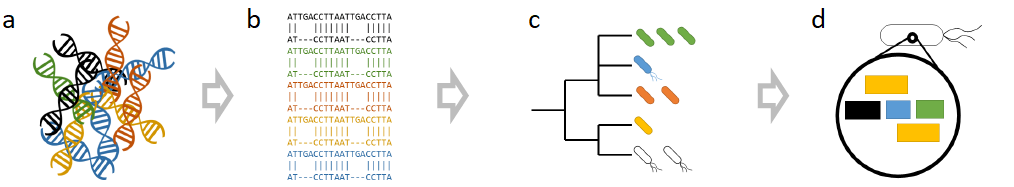
\includegraphics[width=.8\linewidth]{fig/taxonomic_profiler.png}
%     \caption{
%         (a) Raw reads from the sequencing machine are demultiplexed into individual samples. Then, each read is quality controlled with by removing adapters, low quality bases and contaminates such as host reads \cite{consortium_structure_2012}. Optionally, the read pairs can be stitched \cite{magoc_flash:_2011}. (b) The quality-controlled reads are aligned against a database of known genomes to identify each read's most likely source taxon \cite{langmead_fast_2012}. (c) The taxa that are hit are filtered out and summarized at a specific level. These processing steps include last common ancestor assignment \cite{hong_pathoscope_2014}, genome coverage analysis \cite{wood_kraken:_2014}, and redistribution of reads to a specific taxonomic level \cite{lu_bracken:_2017}. (d) After the taxonomic prediction is set, the full functional repertoire of genes is directly observed through a bag-of-genes approach or predicted through a per microbe approach \cite{langille_predictive_2013}.
%     }
%     \label{fig:taxonomic_profiler}
% \end{figure}

%%% fig:shogun_schematic
\begin{figure}[hbt]
    \centering
    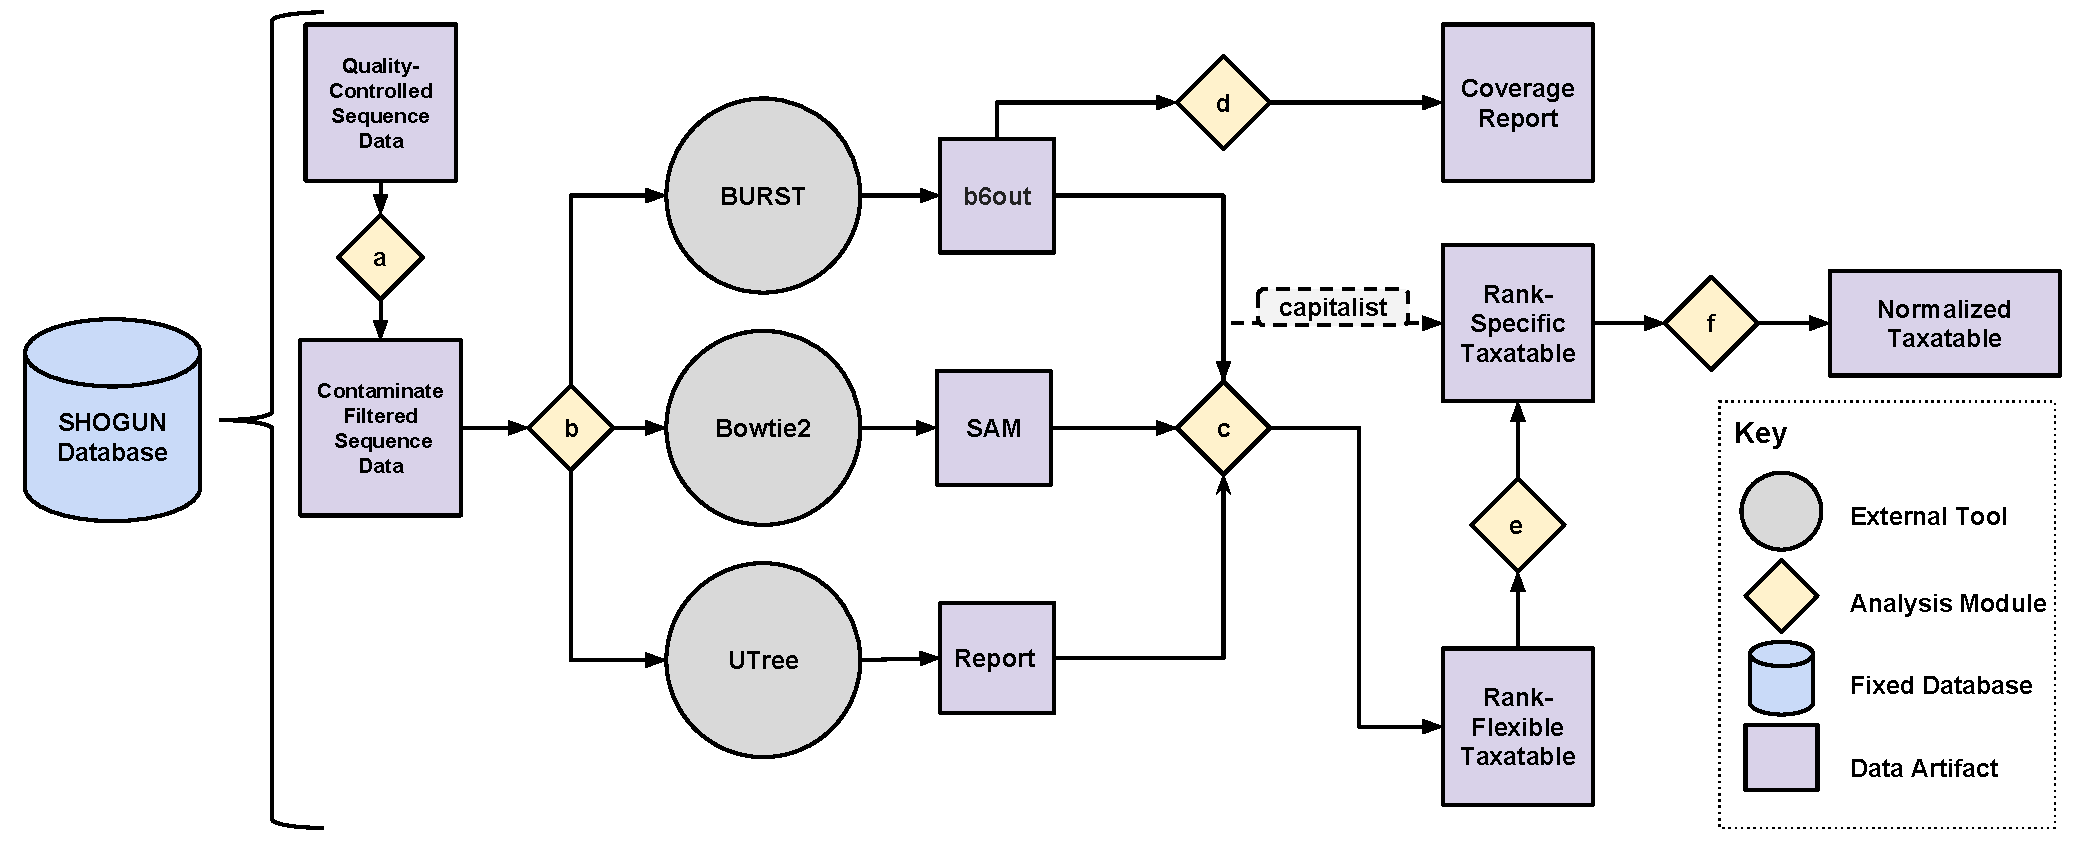
\includegraphics[width=0.8\linewidth]{fig/shogun_schematic.pdf}
    \caption{
        Schematic overview of the shallow-shotgun computational pipeline SHOGUN. For every step in the SHOGUN pipeline, the user must supply the pre-formatted SHOGUN database folder. To run every step shown here in a single command, the user can select the \code{pipeline} subcommand. Otherwise, the analysis modules can be run independently. (a) \code{filter} - The input quality-controlled reads are aligned against the contaminate database using BURST to filter out all reads that hit human associated genome content. (b) \code{align} - The input contaminate filtered reads are aligned against the reference database. The user has the option to select one or all of the three alignment tools BURST, Bowtie2, or UTree. (c) \code{assign\_taxonomy} - Given the data artifacts from a SHOGUN alignment tool, output a Biological Observation Matrix (BIOM) \cite{mcdonald_biological_2012} format taxatable with the rows being rank-flexible taxonomies, the columns are samples, and the entries are counts for each given taxonomy per sample. The alignment tool BURST has two run modes, taxonomy and capitalist. If the capitalist mode is enabled, a rank-specific BIOM file is output instead. (d) \code{coverage} - The output from BURST can be utilized to analyze the coverage of each taxonomy across all samples in your alignment file. This can useful for reducing the number of false positive taxonomies. (e) \code{redistribute} - The rank-flexible taxatable is summarized into a rank-specific taxatable. This summarizes both up and down the taxonomic tree. (f) \code{normalize} - Each sample in the taxatable is normalized to the median depth of all the samples.
    }
    \label{fig:shogun_schematic}
\end{figure}

%%% fig:hmp_beta
\begin{figure}[hbt]
    \centering
    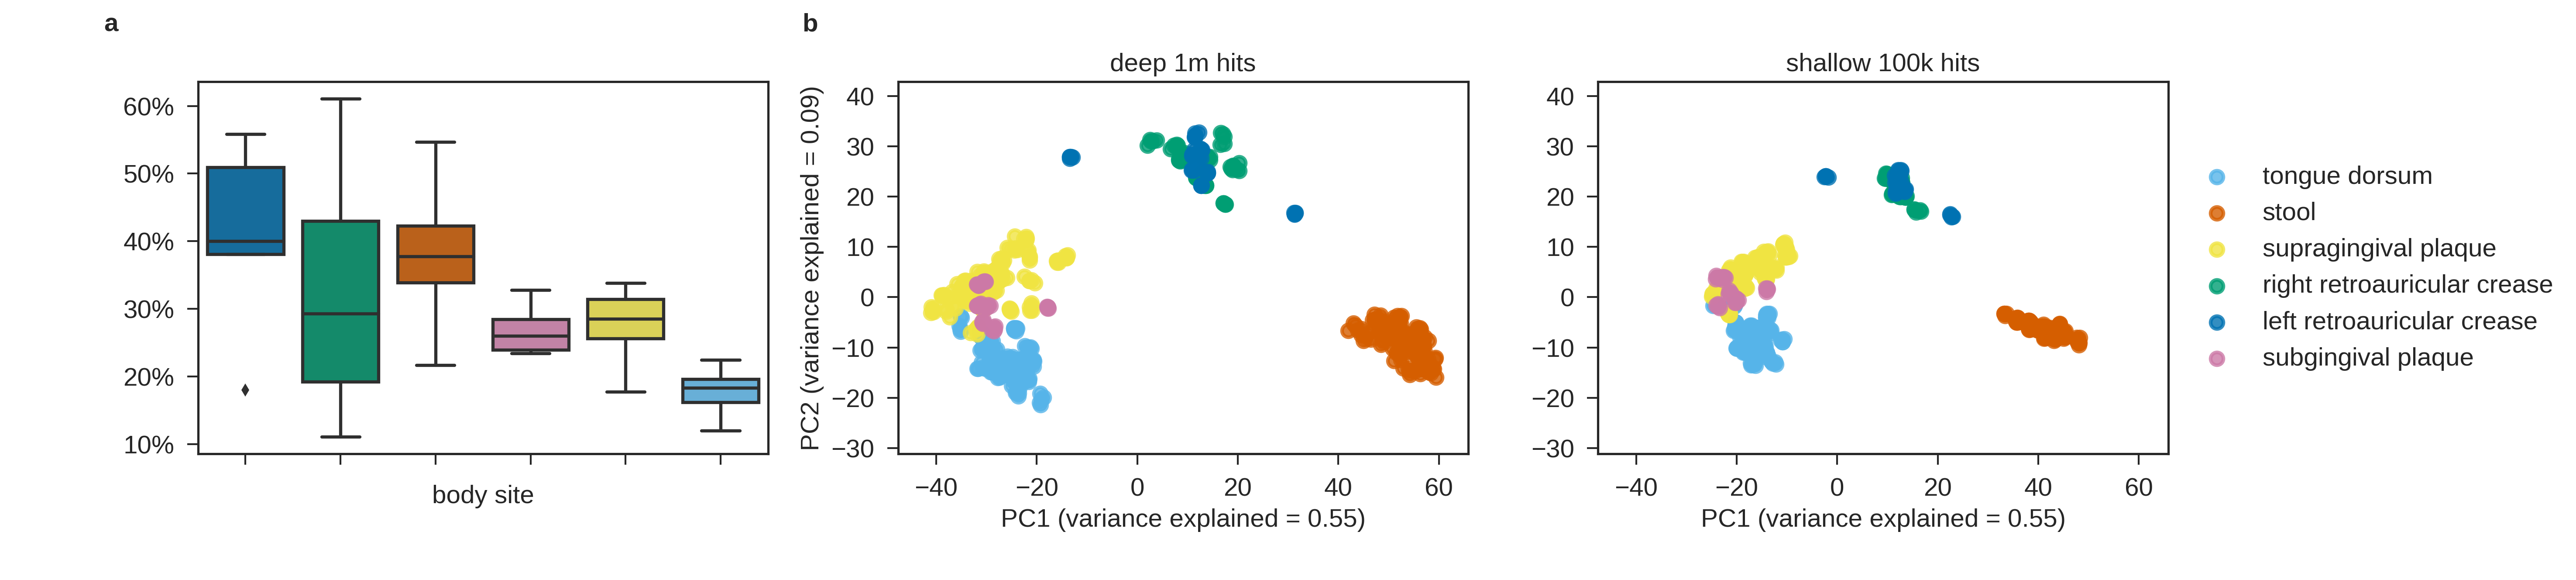
\includegraphics[width=0.8\linewidth]{fig/hmp_beta.png}
    \caption{
        (a) The alignment rate of the sequences to the reference database per body site using BURST capitalist. Most samples aligned at approximately a 25\% rate at 98\% sequence identity to a genome in the reference database. (b) Beta-diversity plots using Euclidean distance on Centered Log-Ratio (CLR) with multiplicate-replacement transformed data. Shown here are the two dimensions that explain the most variance in the data after Principal Components Analysis (PCA). Notice that the groups clearly separate by body sites at both deep- (ADONIS p-value .008**, beta-dispersion p-value=.003**) and shallow-sequencing depths (ADONIS p-value=.02*, beta-dispersion p-value=.01*). 
    }
    \label{fig:hmp_beta}
\end{figure}

%%% fig:hmp_alpha
\begin{figure}[hbt]
    \centering
    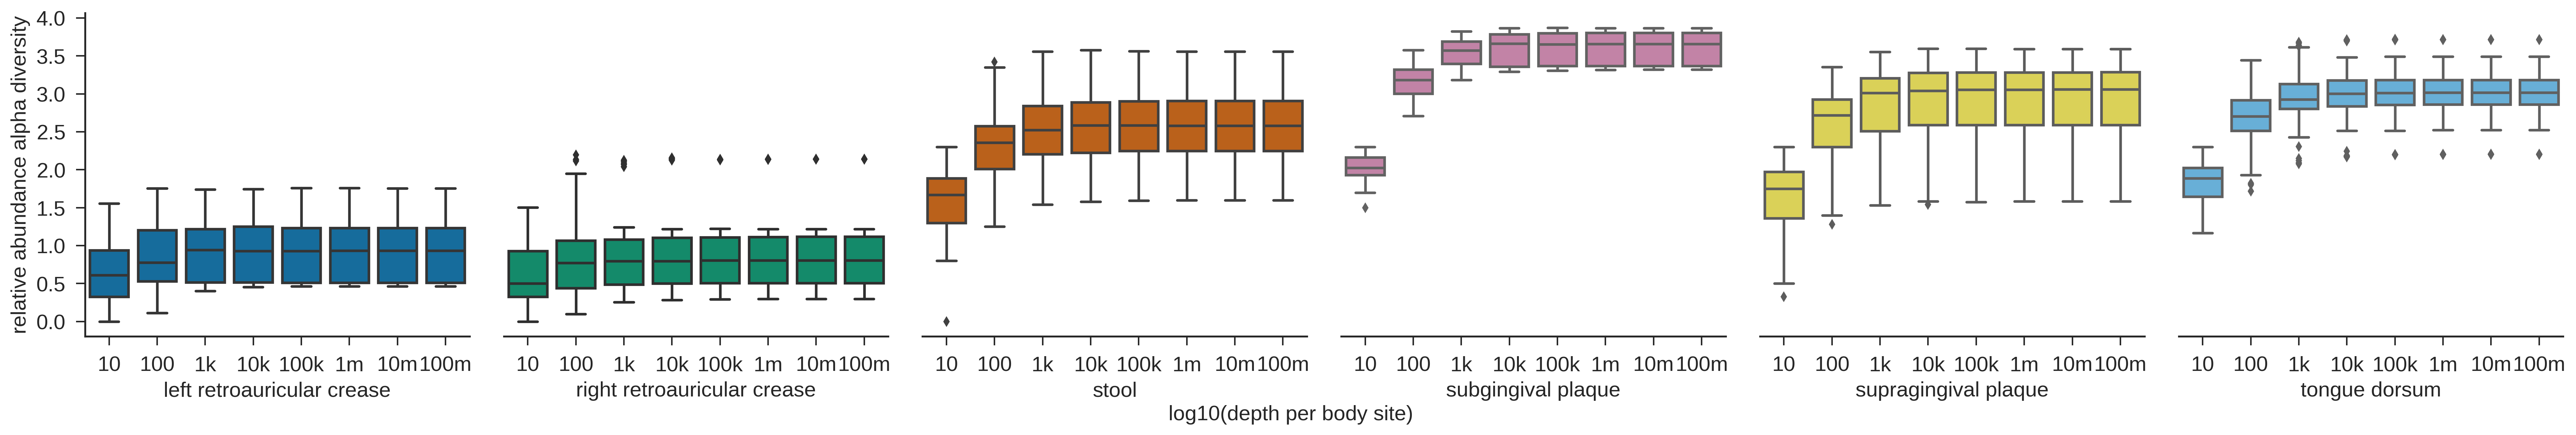
\includegraphics[width=0.8\linewidth]{fig/hmp_alpha.png}
    \caption{
        The alpha-diversity using Shannon index at different bootstrapped depths per body site. Each count vector is summarized using a relative abundance transformation. In all cases, full alpha-diversity is captured between a thousand and ten-thousand counts per sample.
     }
     \label{fig:hmp_alpha}
\end{figure}

% %%% fig:hmp_taxa
% \begin{figure}[hbt]
%     \centering
%     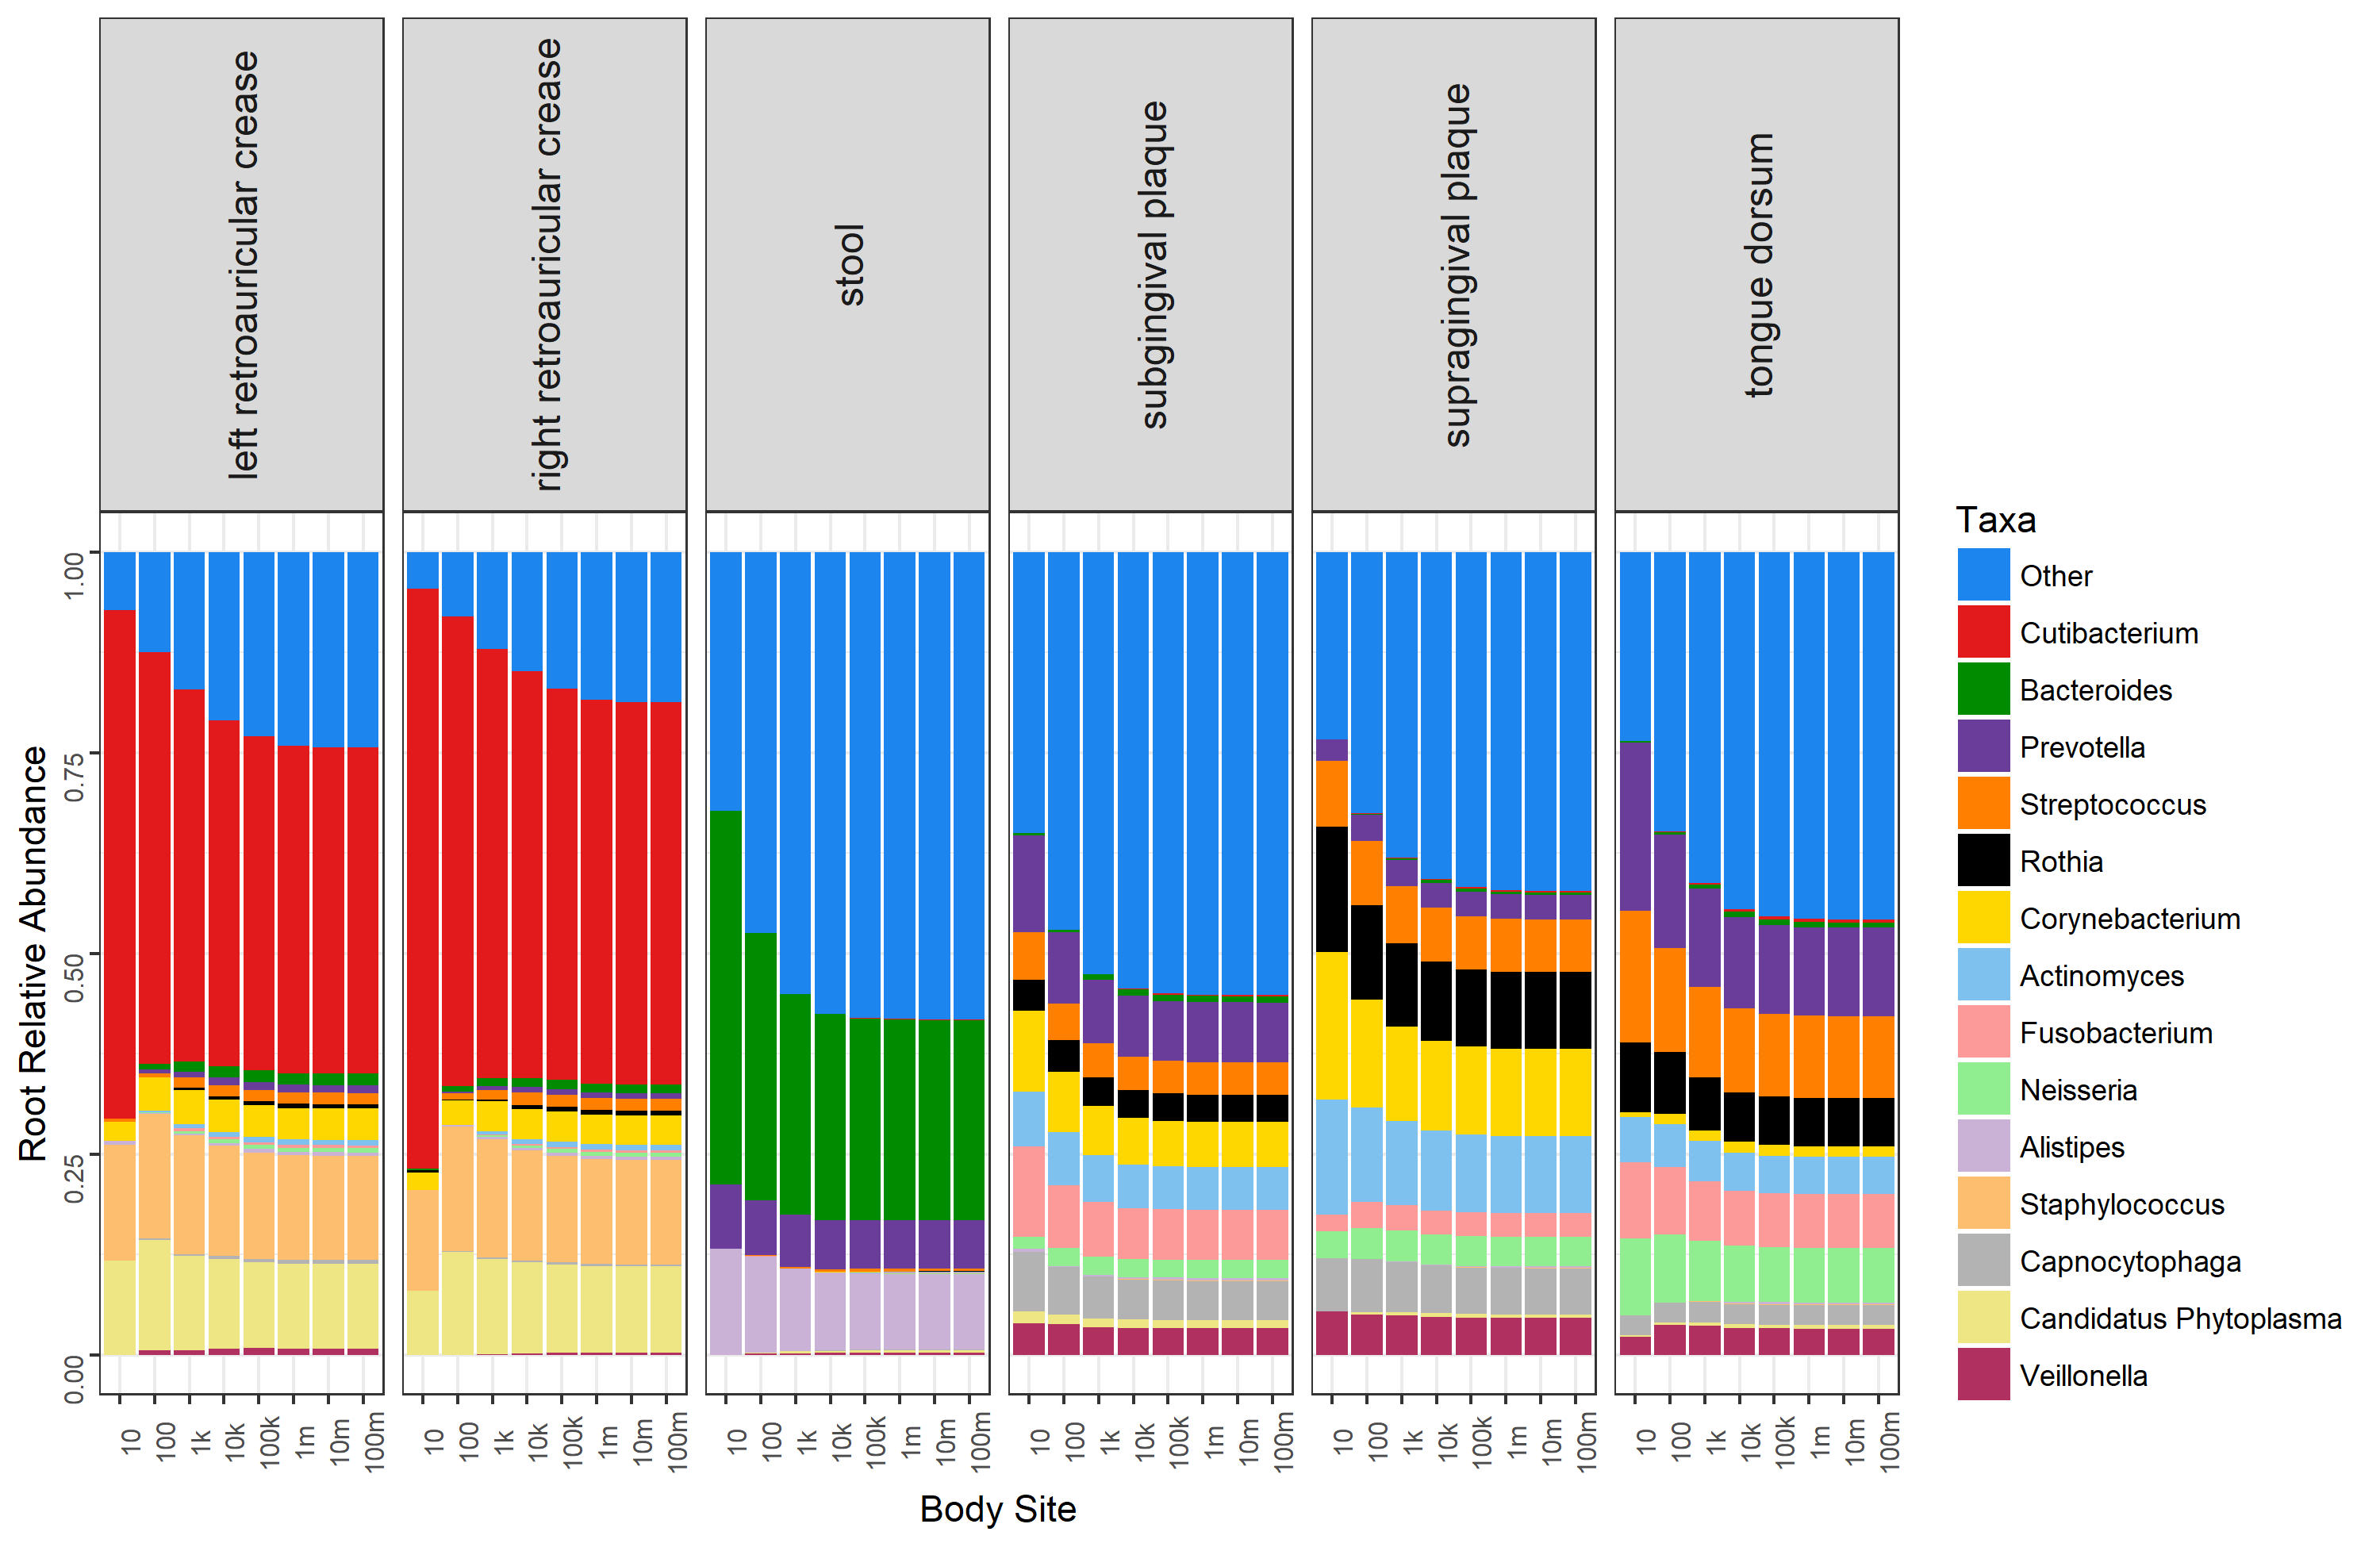
\includegraphics[width=0.99\linewidth]{fig/hmp_taxa.png}
%     \caption{
%         Taxa-summary plots at genus-level (for visualization convenience) stratified by body site by increasing depth. Visually depicted is the transition of the relative abundance vectors to the stabilized full depth relative abundance between a thousand and ten-thousand counts per sample.
%     }
%     \label{fig:hmp_taxa}
% \end{figure}

%%% fig:karlsson2013_f1_combined
\begin{figure}[hbt]
    \centering
    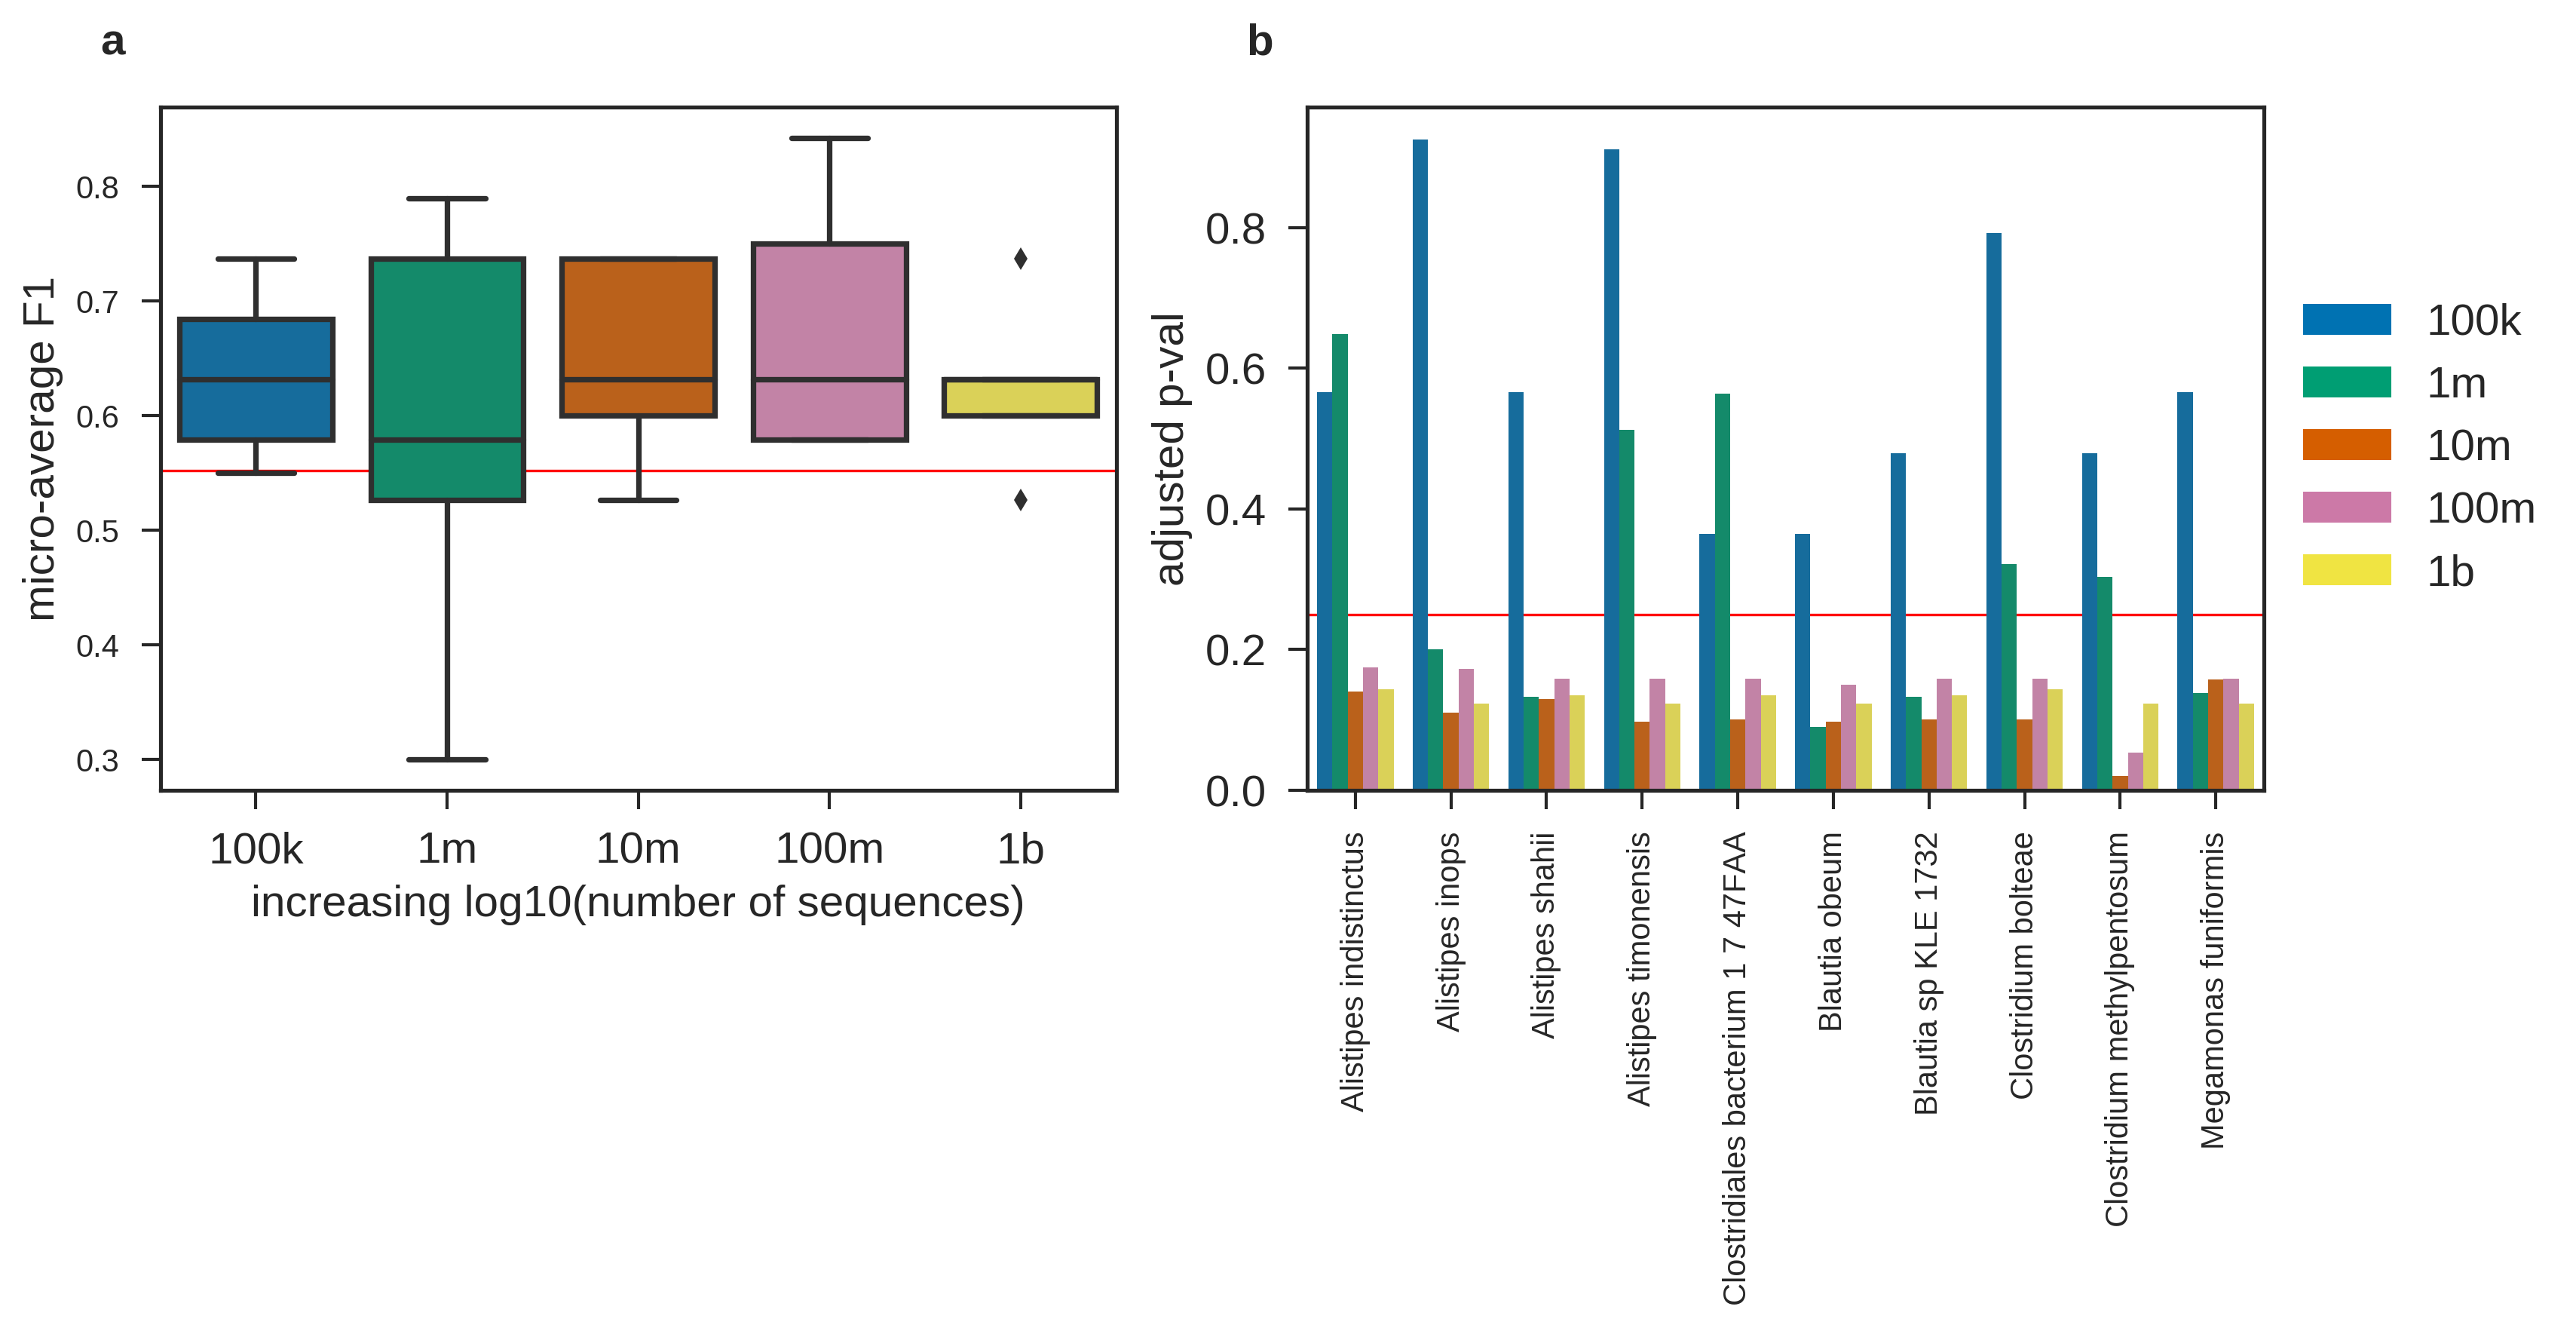
\includegraphics[width=0.8\linewidth]{fig/karlsson2013_f1_combined.png}
    \caption{
        (a) The micro-averaged F1-Score from 10-fold cross-validation on predicting normal glucose tolerance (NGT) versus type-2 diabetes (T2D) on centered log-ration (CLR) multiplicative replacement transformed Karlsson dataset. The classifier used was a Support Vector Machine (SVM) with a linear kernel. The red line is the baseline classifier that predicts majority class (NGT samples = 43, T2D samples = 53). At all subsampled depths, the classifier is able to outperform the baseline classifier verifying the discriminative correlation of microbes with T2D. (b) The Benjamini-Hochberg adjusted Wilcoxon signed-rank p-values for the differentially abundant species between T2D and NGT at varying depths. Displayed are the top ten most differentially abundant species at full depth. The red line is a false-positive rate of 25\%. All species remain significant until a subsampled depth of a thousendth of the original sequences.
    }
    \label{fig:karlsson2013_f1_combined}
\end{figure}

%%% fig:simulations
\begin{figure}[hbt]
    \centering
    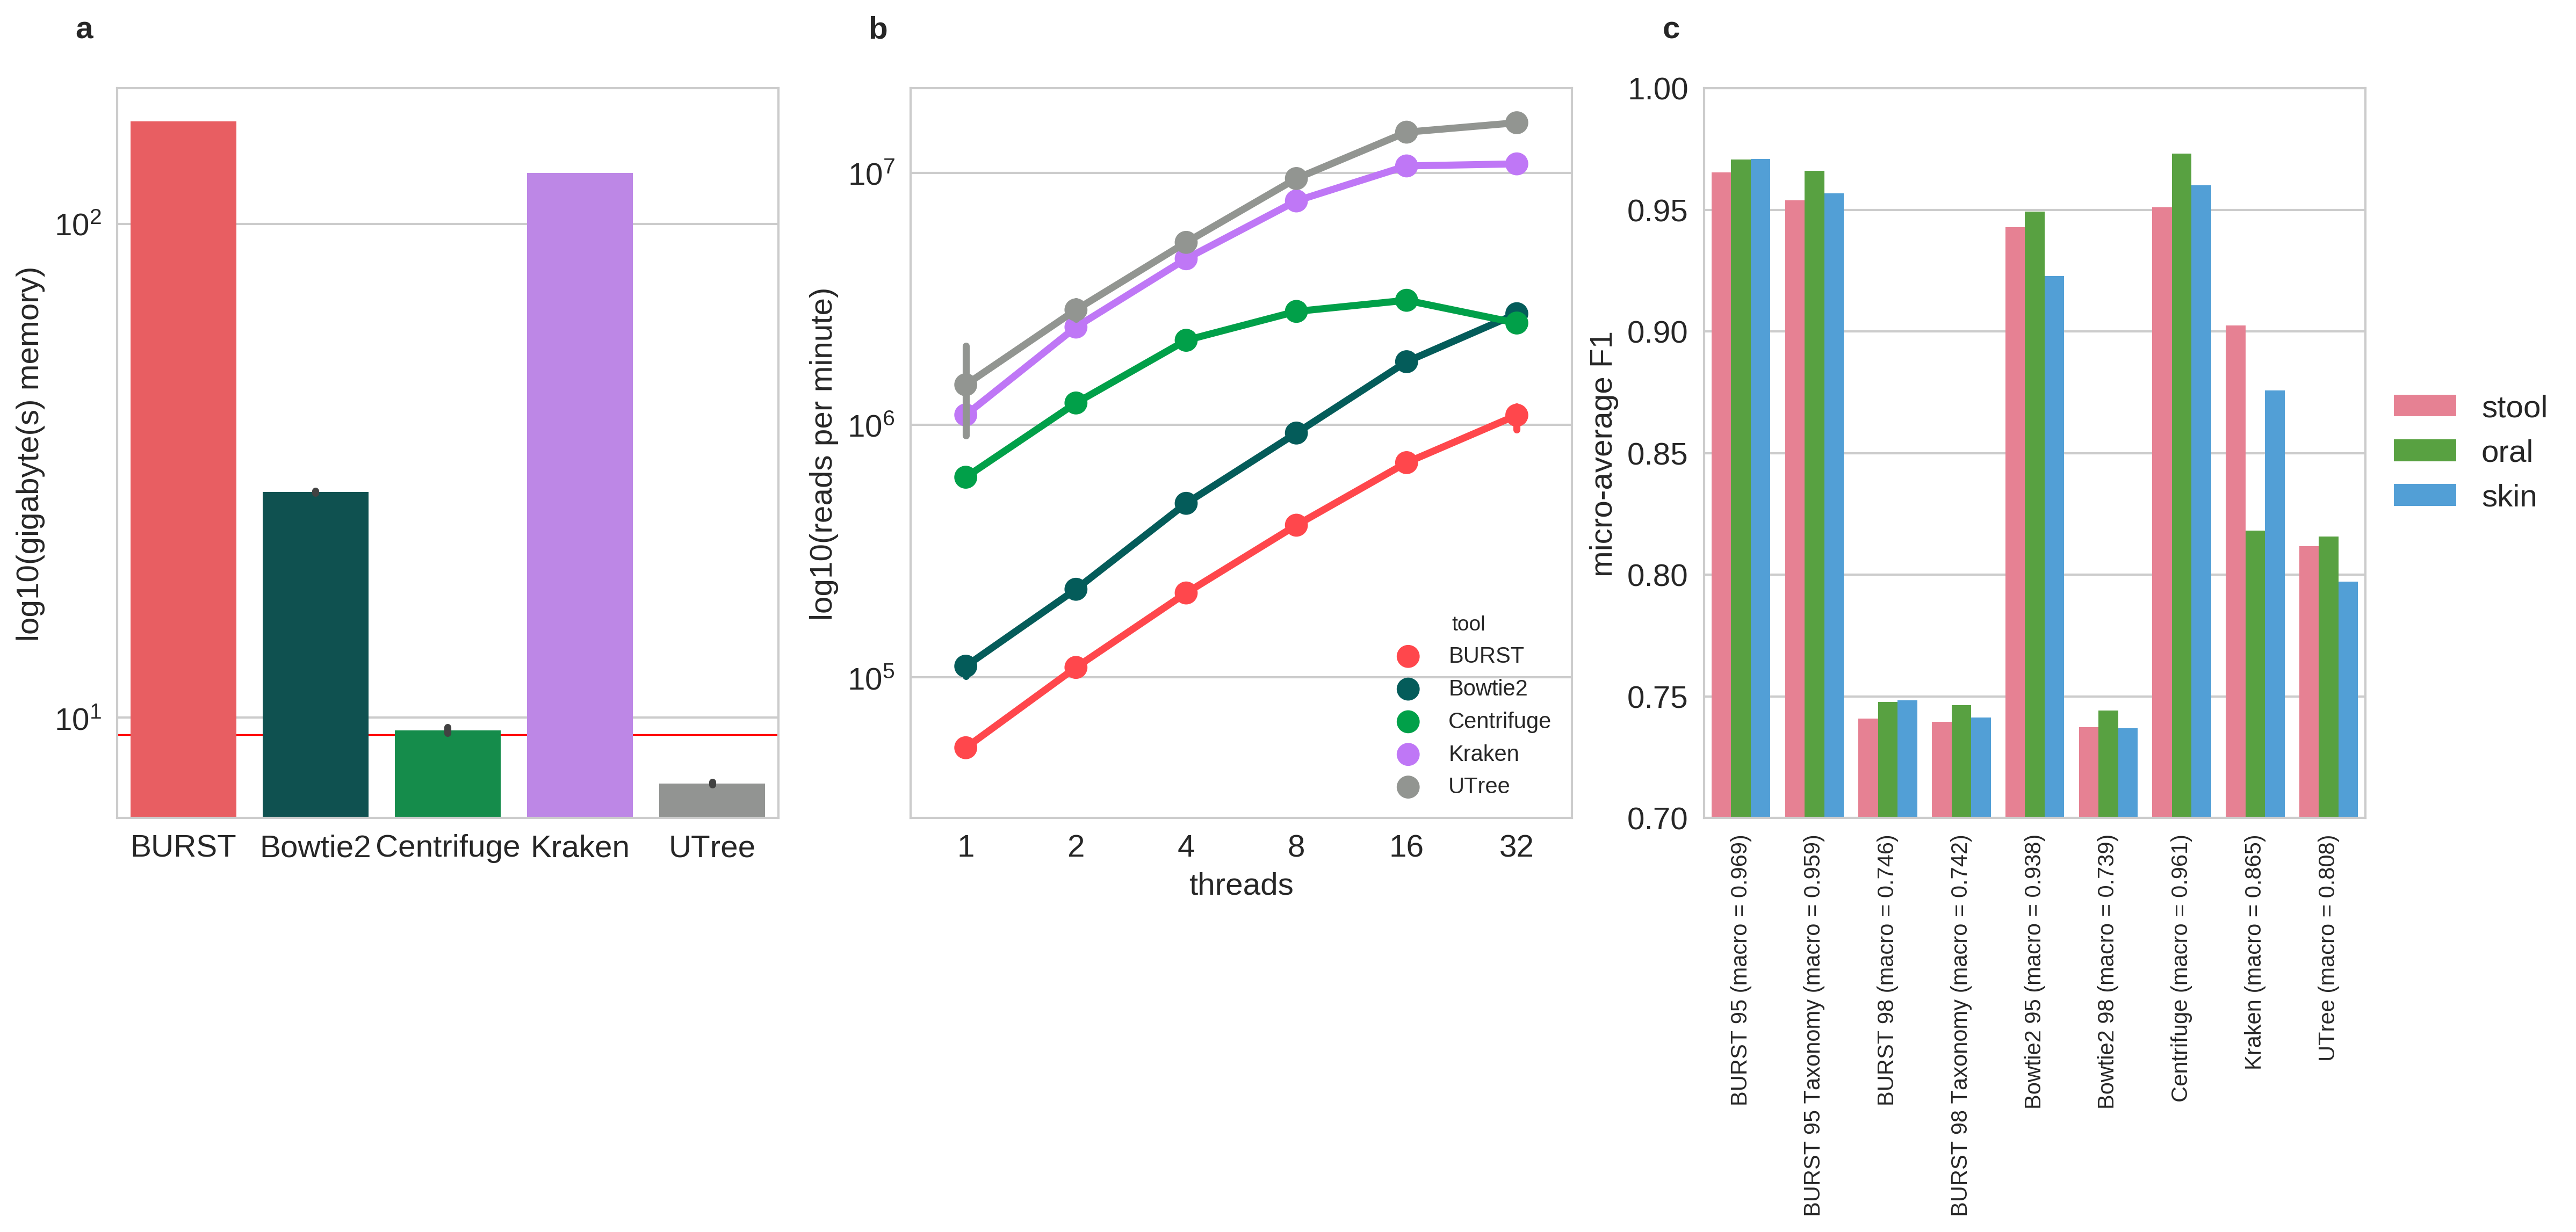
\includegraphics[width=0.8\linewidth]{fig/simulations.png}
    \caption{
        (a) The maximum resident size set (RSS) in Gigabytes of each of the aligners with the Kraken timing dataset. The horizontal red line depicts the size of the original Rep82 database. (b) The scaling and efficiency in reads per minute of each of the aligners across many threads per process. The fastest tools are the alignment free methods Kraken and UTree. Each of the tools scale efficiently across many threads per process. (c) The micro-averaged F1-score of each of the aligners on per read bases on the simulated stool, oral, and skin communities. For the alignment methods, two different thresholds at 95\% and 98\% for alignment identification were set to account for recall bias in highly-divergent reads.
    }
    \label{fig:simulations}
\end{figure}

%%% fig:simulations_js
\begin{figure}[hbt]
    \centering
    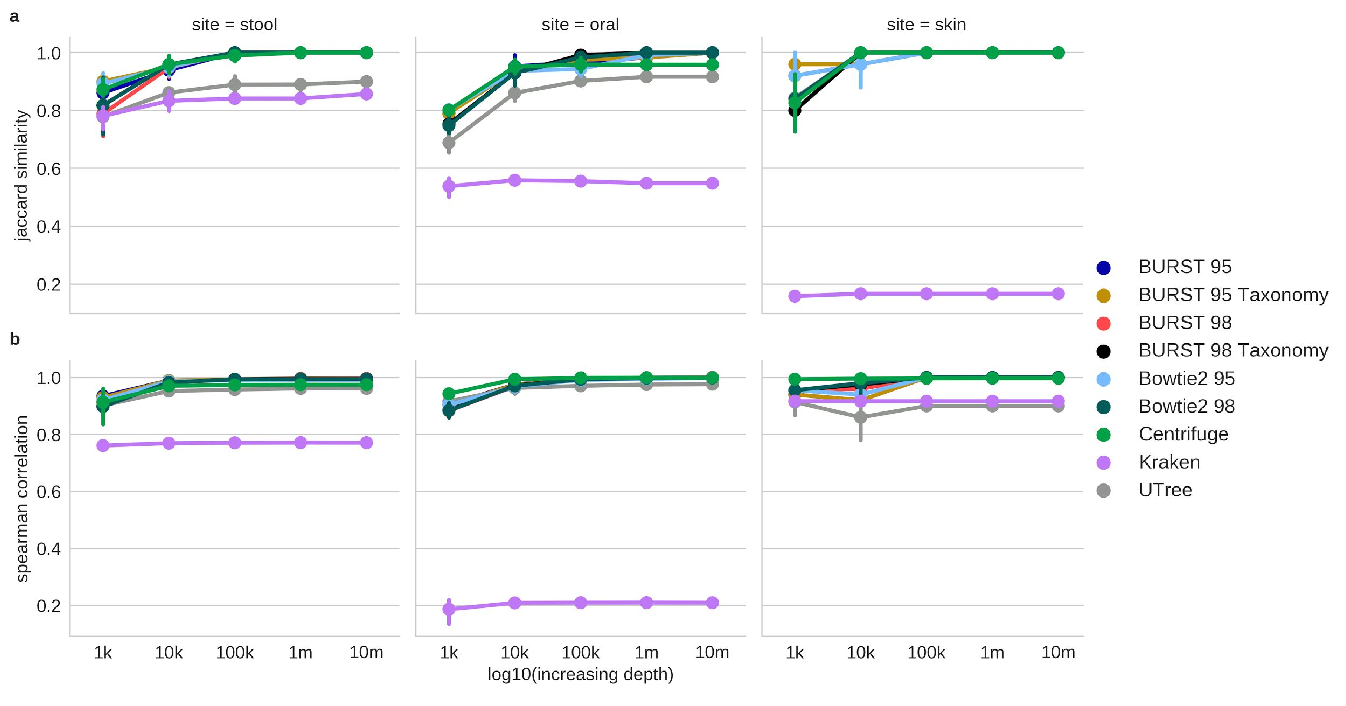
\includegraphics[width=0.8\linewidth]{fig/simulations_js.pdf}
    \caption{
          (a) Rarefaction curves of Jaccard similarity of known species and predicted species for each of the alignment tools on the simulated stool, oral, and skin communities. For most tools, all species are identified between ten-thousand and a hundred thousand reads. (b) The rarefaction curves of Spearman correlation of the tools predicted community with the known community for the simulated dataset. This shows that not only are the correct species identified, but they are also in the correct abundances. 
    }
    \label{fig:simulations_js}
\end{figure}

%%% tab:database_stats
\begin{table}[hbt]
  \centering
  \begin{tabular}{l|r|r}
      \textit{Kingdom} & \textit{Number of Genomes} & \textit{Megabase pairs (Mbp)} \\ \hline
      Archaea & 238 & 627,101.26\\ \hline
      Bacteria & 4,884 & 19,308,087.26\\ \hline
      Plasmid & 614 & 198,476.94\\ \hline
      Viroids & 46 & 15.50\\ \hline
      Viruses & 7,194 & 253,668.36\\ \hline \hline
      \textbf{Total} & \textbf{12,976} & \textbf{20,387,349.32}\\ 
  \end{tabular}
  \caption{
        The number of strains and megabase pairs for each kingdom for all representative Archaea, Bacteria, Plasmid, Viroids and Virus sequences in RefSeq version 82 (Rep82). Each entry in the database is assigned a unique taxonomic string identifier at each level in the taxonomic tree down to strain. An example taxonomic annotation for humans is \code{k\_\_Eukaryota;p\_\_Chordata;c\_\_Mammalia;o\_\_Primates;f\_\_Hominidae;g\_\_Homo;s\_\_Homo\_sapiens;t\_\_}. Each strain is a given a unique entry so that BURST capitalist properly disambiguates reads that hit multiple strains for proper taxonomic profiling and coverage analysis. 
  }
  \label{tab:database_stats}
\end{table}

% Table generated by Excel2LaTeX
%%% tab:discussion
\begin{table}[htbp]
      \centering
      \begin{tabular}{rrll}
      \multicolumn{1}{l}{\textit{Approach}} & \multicolumn{1}{l}{\textit{Examples}} & \textit{Pros} & \textit{Cons} \\
      \midrule
      \midrule
      \multicolumn{1}{l}{\textbf{Last Common Ancestor Alignment}} & \multicolumn{1}{l}{Bowtie2 Taxonomy} & Highest Precision & High RAM \\
            & \multicolumn{1}{l}{BURST Taxonomy} &       & \multicolumn{1}{p{9.5em}}{Slow} \\
            &       &       & No coverage analysis \\
      \midrule
      \multicolumn{1}{l}{\textbf{Exhaustive Alignment}} & \multicolumn{1}{l}{BURST Capitalist} & Highest F1 Accuracy & High RAM \\
            &       & Highest Recall & Slow \\
      \midrule
      \multicolumn{1}{l}{\textbf{Marker Gene}$^\dagger$} & \multicolumn{1}{l}{Metaphlan} & Low RAM & Sparse Database \\
            &       & Fast  &  \\
      \midrule
      \multicolumn{1}{l}{\textbf{Exact K-mers}} &       & Fastest & No coverage analysis \\
            &       &       & Sensitive to indels \\
      \cdashlinelr{2-4}
            & \multicolumn{1}{l}{Kraken} &       & High RAM \\
            &       &       & Large Database \\
      \cdashlinelr{2-4}
            & \multicolumn{1}{l}{Utree} & Lowest RAM &  \\
            &       & Smallest Database &  \\
      \midrule
      \multicolumn{1}{l}{\textbf{Longest Common Substring}} & \multicolumn{1}{l}{Centrifuge} & Fast  & No coverage analysis \\
            &       & Low RAM & Sensitive to indels \\
      \bottomrule
      \multicolumn{4}{l}{$^\dagger$\footnotesize{ Marker gene taxonomic profilers were not evaluated in this study due to complexity of creating a database and low alignment rates.}}
      \end{tabular}%
      \caption{
            Summarization of the many tools tested in this paper for shallow-shotgun sequencing. While this list is not comprehensive, we recommend using any tools in the approaches listed as legitimate options for analysis of shallow-shotgun data except for a marker gene$^\dagger$ approach. From the tools surveyed, we found that BURST capitalist returns the most accurate results if properly tuned at the cost of high RAM usage and compute time. If computer resources is a concern, we recommend using either UTree on a computer with over 8GB RAM or Centrifuge on a computer with over 16GB RAM.
      }
      \label{tab:discussion}
\end{table}


\newpage

\section{Data Availability}

\subsection{Rep82}
The catalog for the genomes is available at \url{ftp://ftp.ncbi.nlm.nih.gov/refseq/release/release-catalog/archive/}, and the release statistics notes are available at \url{ftp://ftp.ncbi.nlm.nih.gov/refseq/release/release-notes/archive/RefSeq-release82.txt}.

\subsection{GRCh38}
The download for GRCh38 is available at \url{ftp://ftp.ncbi.nlm.nih.gov/genomes/all/GCA/000/001/405/GCA_000001405.15_GRCh38/seqs_for_alignment_pipelines.ucsc_ids/GCA_000001405.15_GRCh38_no_alt_analysis_set.fna.gz}.

\subsection{Human Microbiome Project}
All data is available through the ftp website located at \url{ftp://public-ftp.ihmpdcc.org/HMASM/WGS/}.

\subsection{Karlsson Dataset}
Data for the Karlsson dataset is available in the Sequence Read Archive (sra) under accession code ERP002469.

\subsection{Kraken Timing}
The Kraken timing dataset is available at \url{https://ccb.jhu.edu/software/kraken/dl/timing.tgz}.

\subsection{SHOGUN}
The analysis tool SHOGUN is available at \url{https://github.com/knights-lab/SHOGUN}. All analysis for this paper is available at \url{https://github.com/knights-lab/analysis_SHOGUN}.

\subsection{UTree}
The taxonomic profiling tool UTree is available at \url{https://github.com/knights-lab/UTree}.

\subsection{BURST}
The taxonomic profiling tool BURST is available at \url{https://github.com/knights-lab/BURST}.


\newpage

\bibliographystyle{ACM-Reference-Format}
\bibliography{Zotero}

\newpage

%%% fig:taxonomic_profiler
% \begin{figure}[hbt]
%     \centering
%     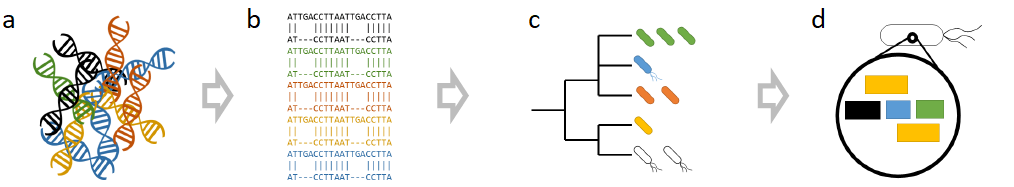
\includegraphics[width=.8\linewidth]{fig/taxonomic_profiler.png}
%     \caption{
%         (a) Raw reads from the sequencing machine are demultiplexed into individual samples. Then, each read is quality controlled with by removing adapters, low quality bases and contaminates such as host reads \cite{consortium_structure_2012}. Optionally, the read pairs can be stitched \cite{magoc_flash:_2011}. (b) The quality-controlled reads are aligned against a database of known genomes to identify each read's most likely source taxon \cite{langmead_fast_2012}. (c) The taxa that are hit are filtered out and summarized at a specific level. These processing steps include last common ancestor assignment \cite{hong_pathoscope_2014}, genome coverage analysis \cite{wood_kraken:_2014}, and redistribution of reads to a specific taxonomic level \cite{lu_bracken:_2017}. (d) After the taxonomic prediction is set, the full functional repertoire of genes is directly observed through a bag-of-genes approach or predicted through a per microbe approach \cite{langille_predictive_2013}.
%     }
%     \label{fig:taxonomic_profiler}
% \end{figure}

%%% fig:shogun_schematic
\begin{figure}[hbt]
    \centering
    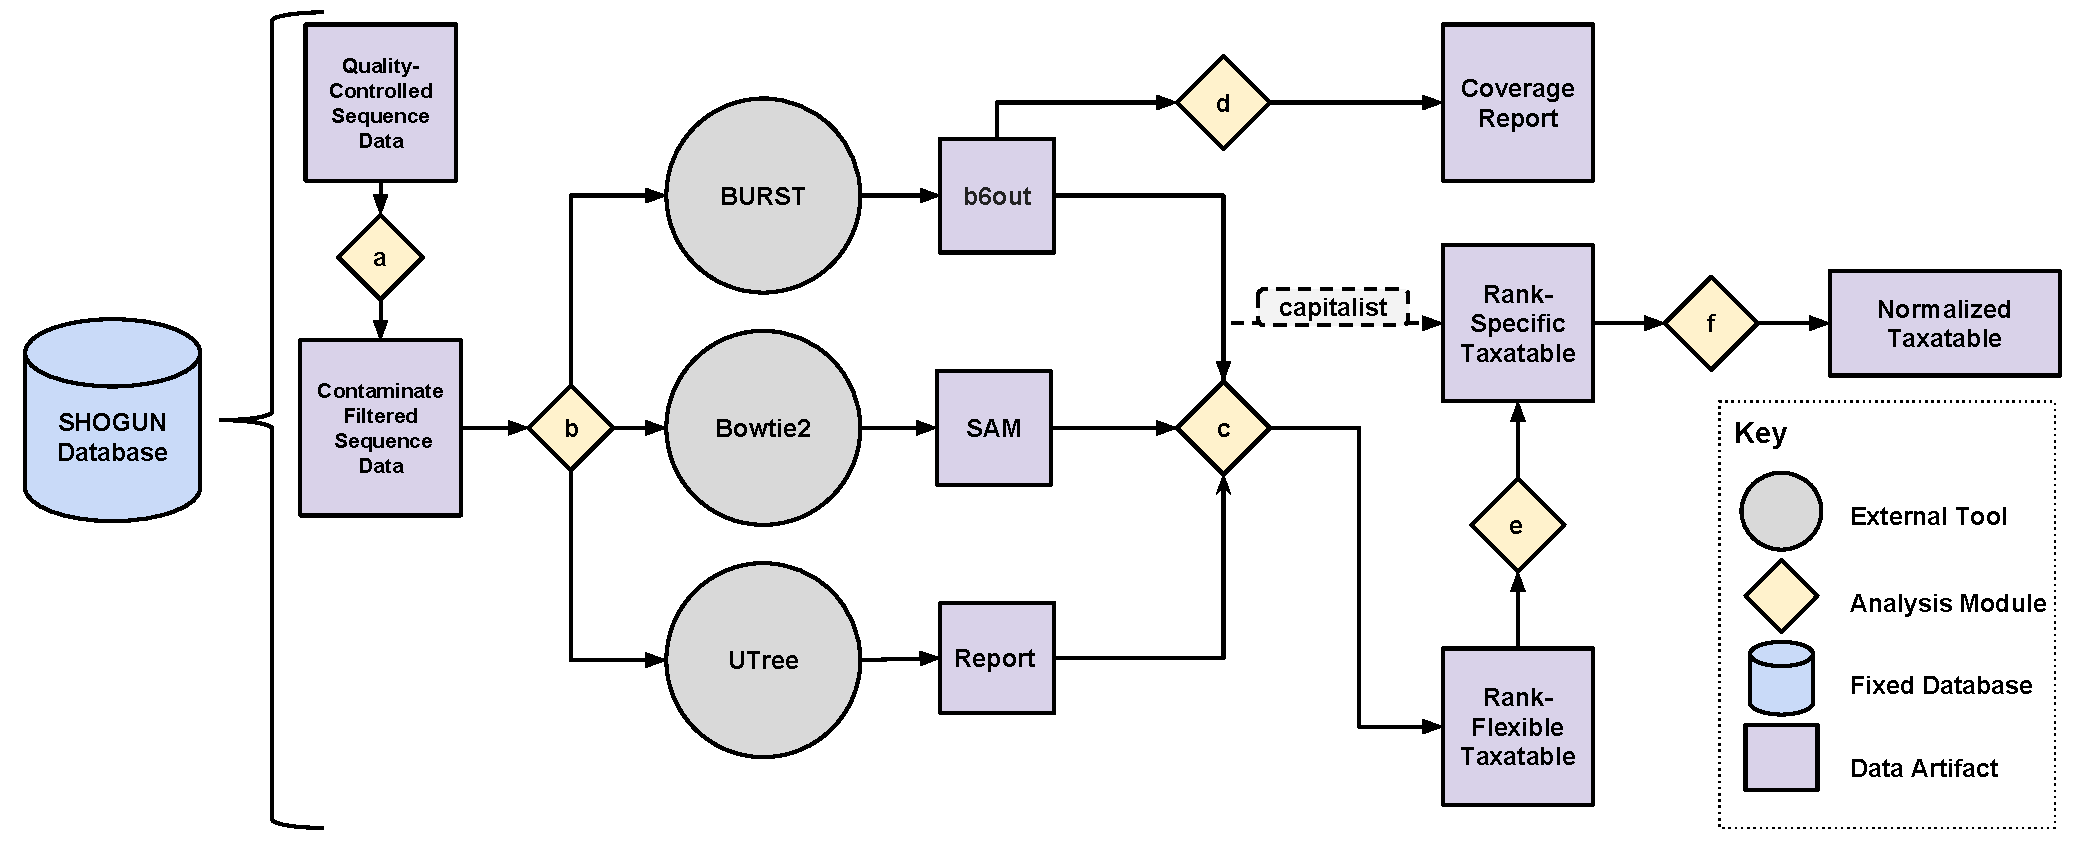
\includegraphics[width=0.8\linewidth]{fig/shogun_schematic.pdf}
    \caption{
        Schematic overview of the shallow-shotgun computational pipeline SHOGUN. For every step in the SHOGUN pipeline, the user must supply the pre-formatted SHOGUN database folder. To run every step shown here in a single command, the user can select the \code{pipeline} subcommand. Otherwise, the analysis modules can be run independently. (a) \code{filter} - The input quality-controlled reads are aligned against the contaminate database using BURST to filter out all reads that hit human associated genome content. (b) \code{align} - The input contaminate filtered reads are aligned against the reference database. The user has the option to select one or all of the three alignment tools BURST, Bowtie2, or UTree. (c) \code{assign\_taxonomy} - Given the data artifacts from a SHOGUN alignment tool, output a Biological Observation Matrix (BIOM) \cite{mcdonald_biological_2012} format taxatable with the rows being rank-flexible taxonomies, the columns are samples, and the entries are counts for each given taxonomy per sample. The alignment tool BURST has two run modes, taxonomy and capitalist. If the capitalist mode is enabled, a rank-specific BIOM file is output instead. (d) \code{coverage} - The output from BURST can be utilized to analyze the coverage of each taxonomy across all samples in your alignment file. This can useful for reducing the number of false positive taxonomies. (e) \code{redistribute} - The rank-flexible taxatable is summarized into a rank-specific taxatable. This summarizes both up and down the taxonomic tree. (f) \code{normalize} - Each sample in the taxatable is normalized to the median depth of all the samples.
    }
    \label{fig:shogun_schematic}
\end{figure}

%%% fig:hmp_beta
\begin{figure}[hbt]
    \centering
    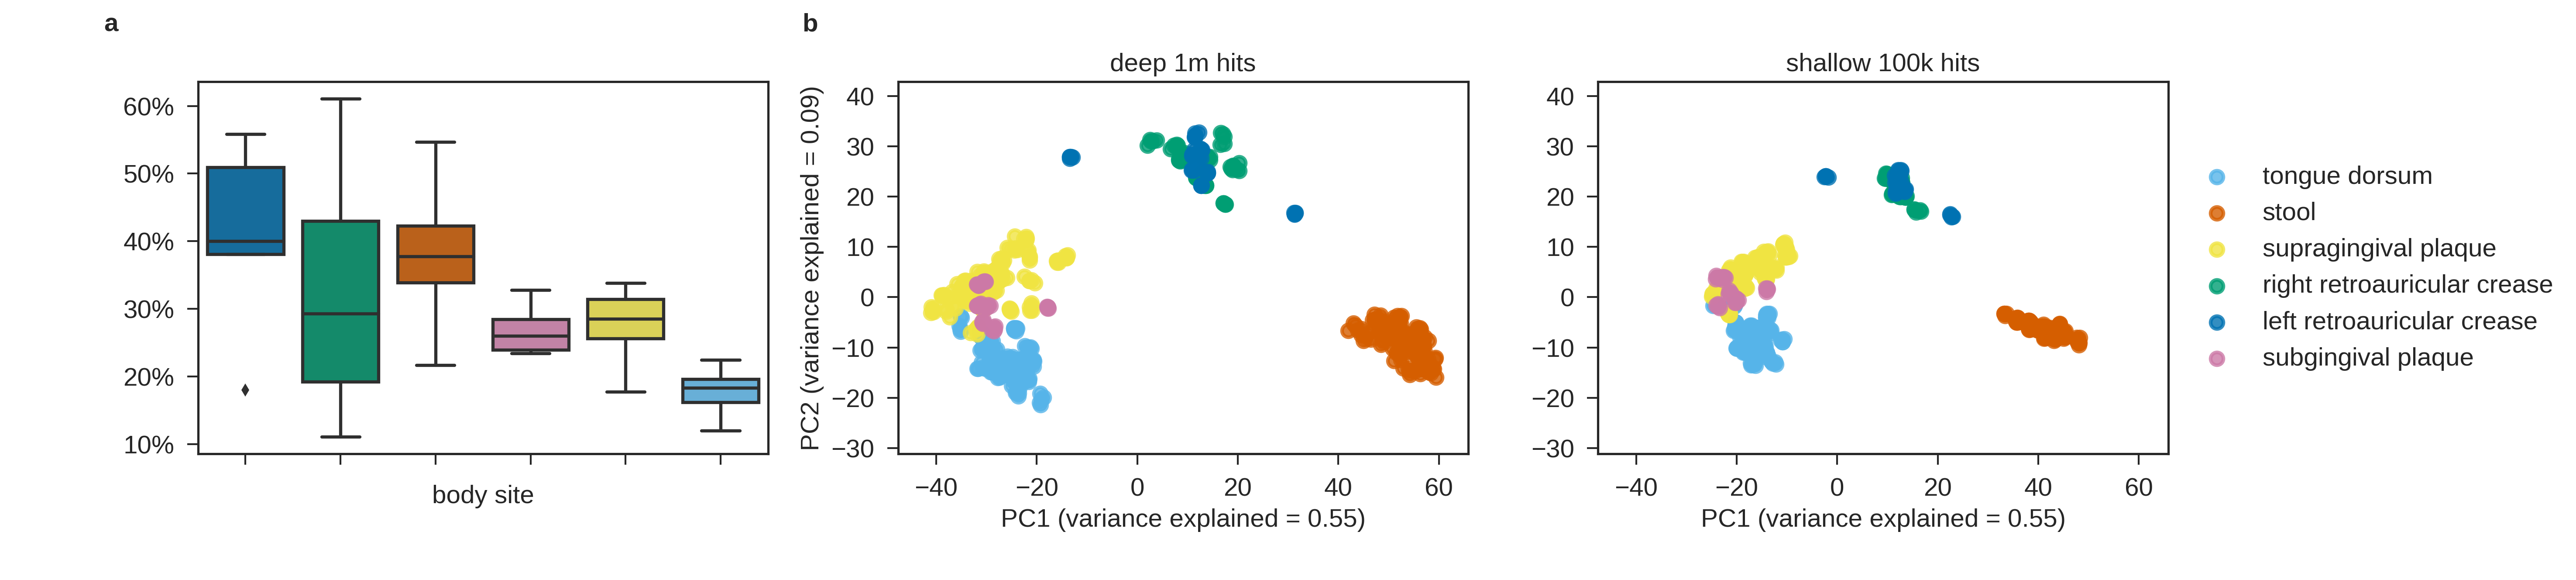
\includegraphics[width=0.8\linewidth]{fig/hmp_beta.png}
    \caption{
        (a) The alignment rate of the sequences to the reference database per body site using BURST capitalist. Most samples aligned at approximately a 25\% rate at 98\% sequence identity to a genome in the reference database. (b) Beta-diversity plots using Euclidean distance on Centered Log-Ratio (CLR) with multiplicate-replacement transformed data. Shown here are the two dimensions that explain the most variance in the data after Principal Components Analysis (PCA). Notice that the groups clearly separate by body sites at both deep- (ADONIS p-value .008**, beta-dispersion p-value=.003**) and shallow-sequencing depths (ADONIS p-value=.02*, beta-dispersion p-value=.01*). 
    }
    \label{fig:hmp_beta}
\end{figure}

%%% fig:hmp_alpha
\begin{figure}[hbt]
    \centering
    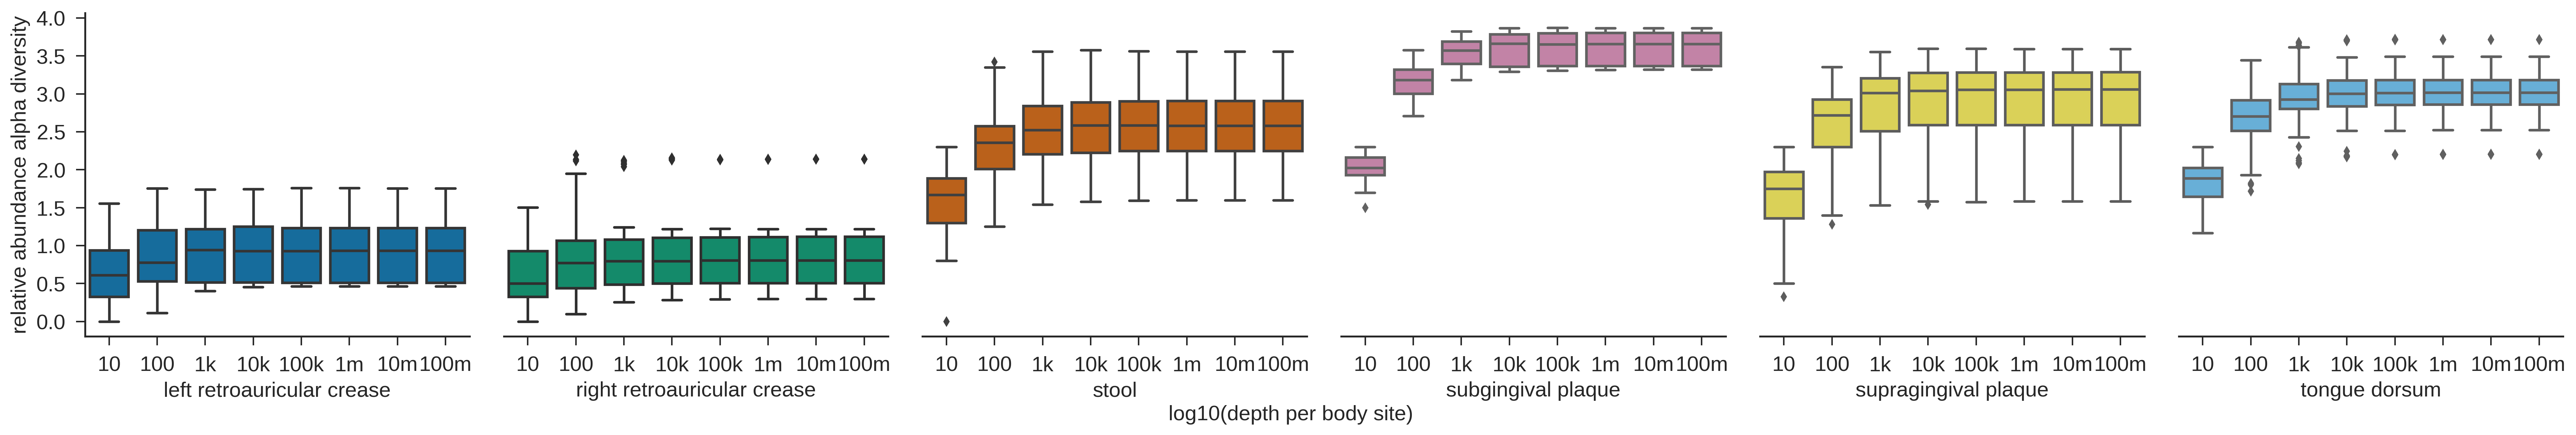
\includegraphics[width=0.8\linewidth]{fig/hmp_alpha.png}
    \caption{
        The alpha-diversity using Shannon index at different bootstrapped depths per body site. Each count vector is summarized using a relative abundance transformation. In all cases, full alpha-diversity is captured between a thousand and ten-thousand counts per sample.
     }
     \label{fig:hmp_alpha}
\end{figure}

% %%% fig:hmp_taxa
% \begin{figure}[hbt]
%     \centering
%     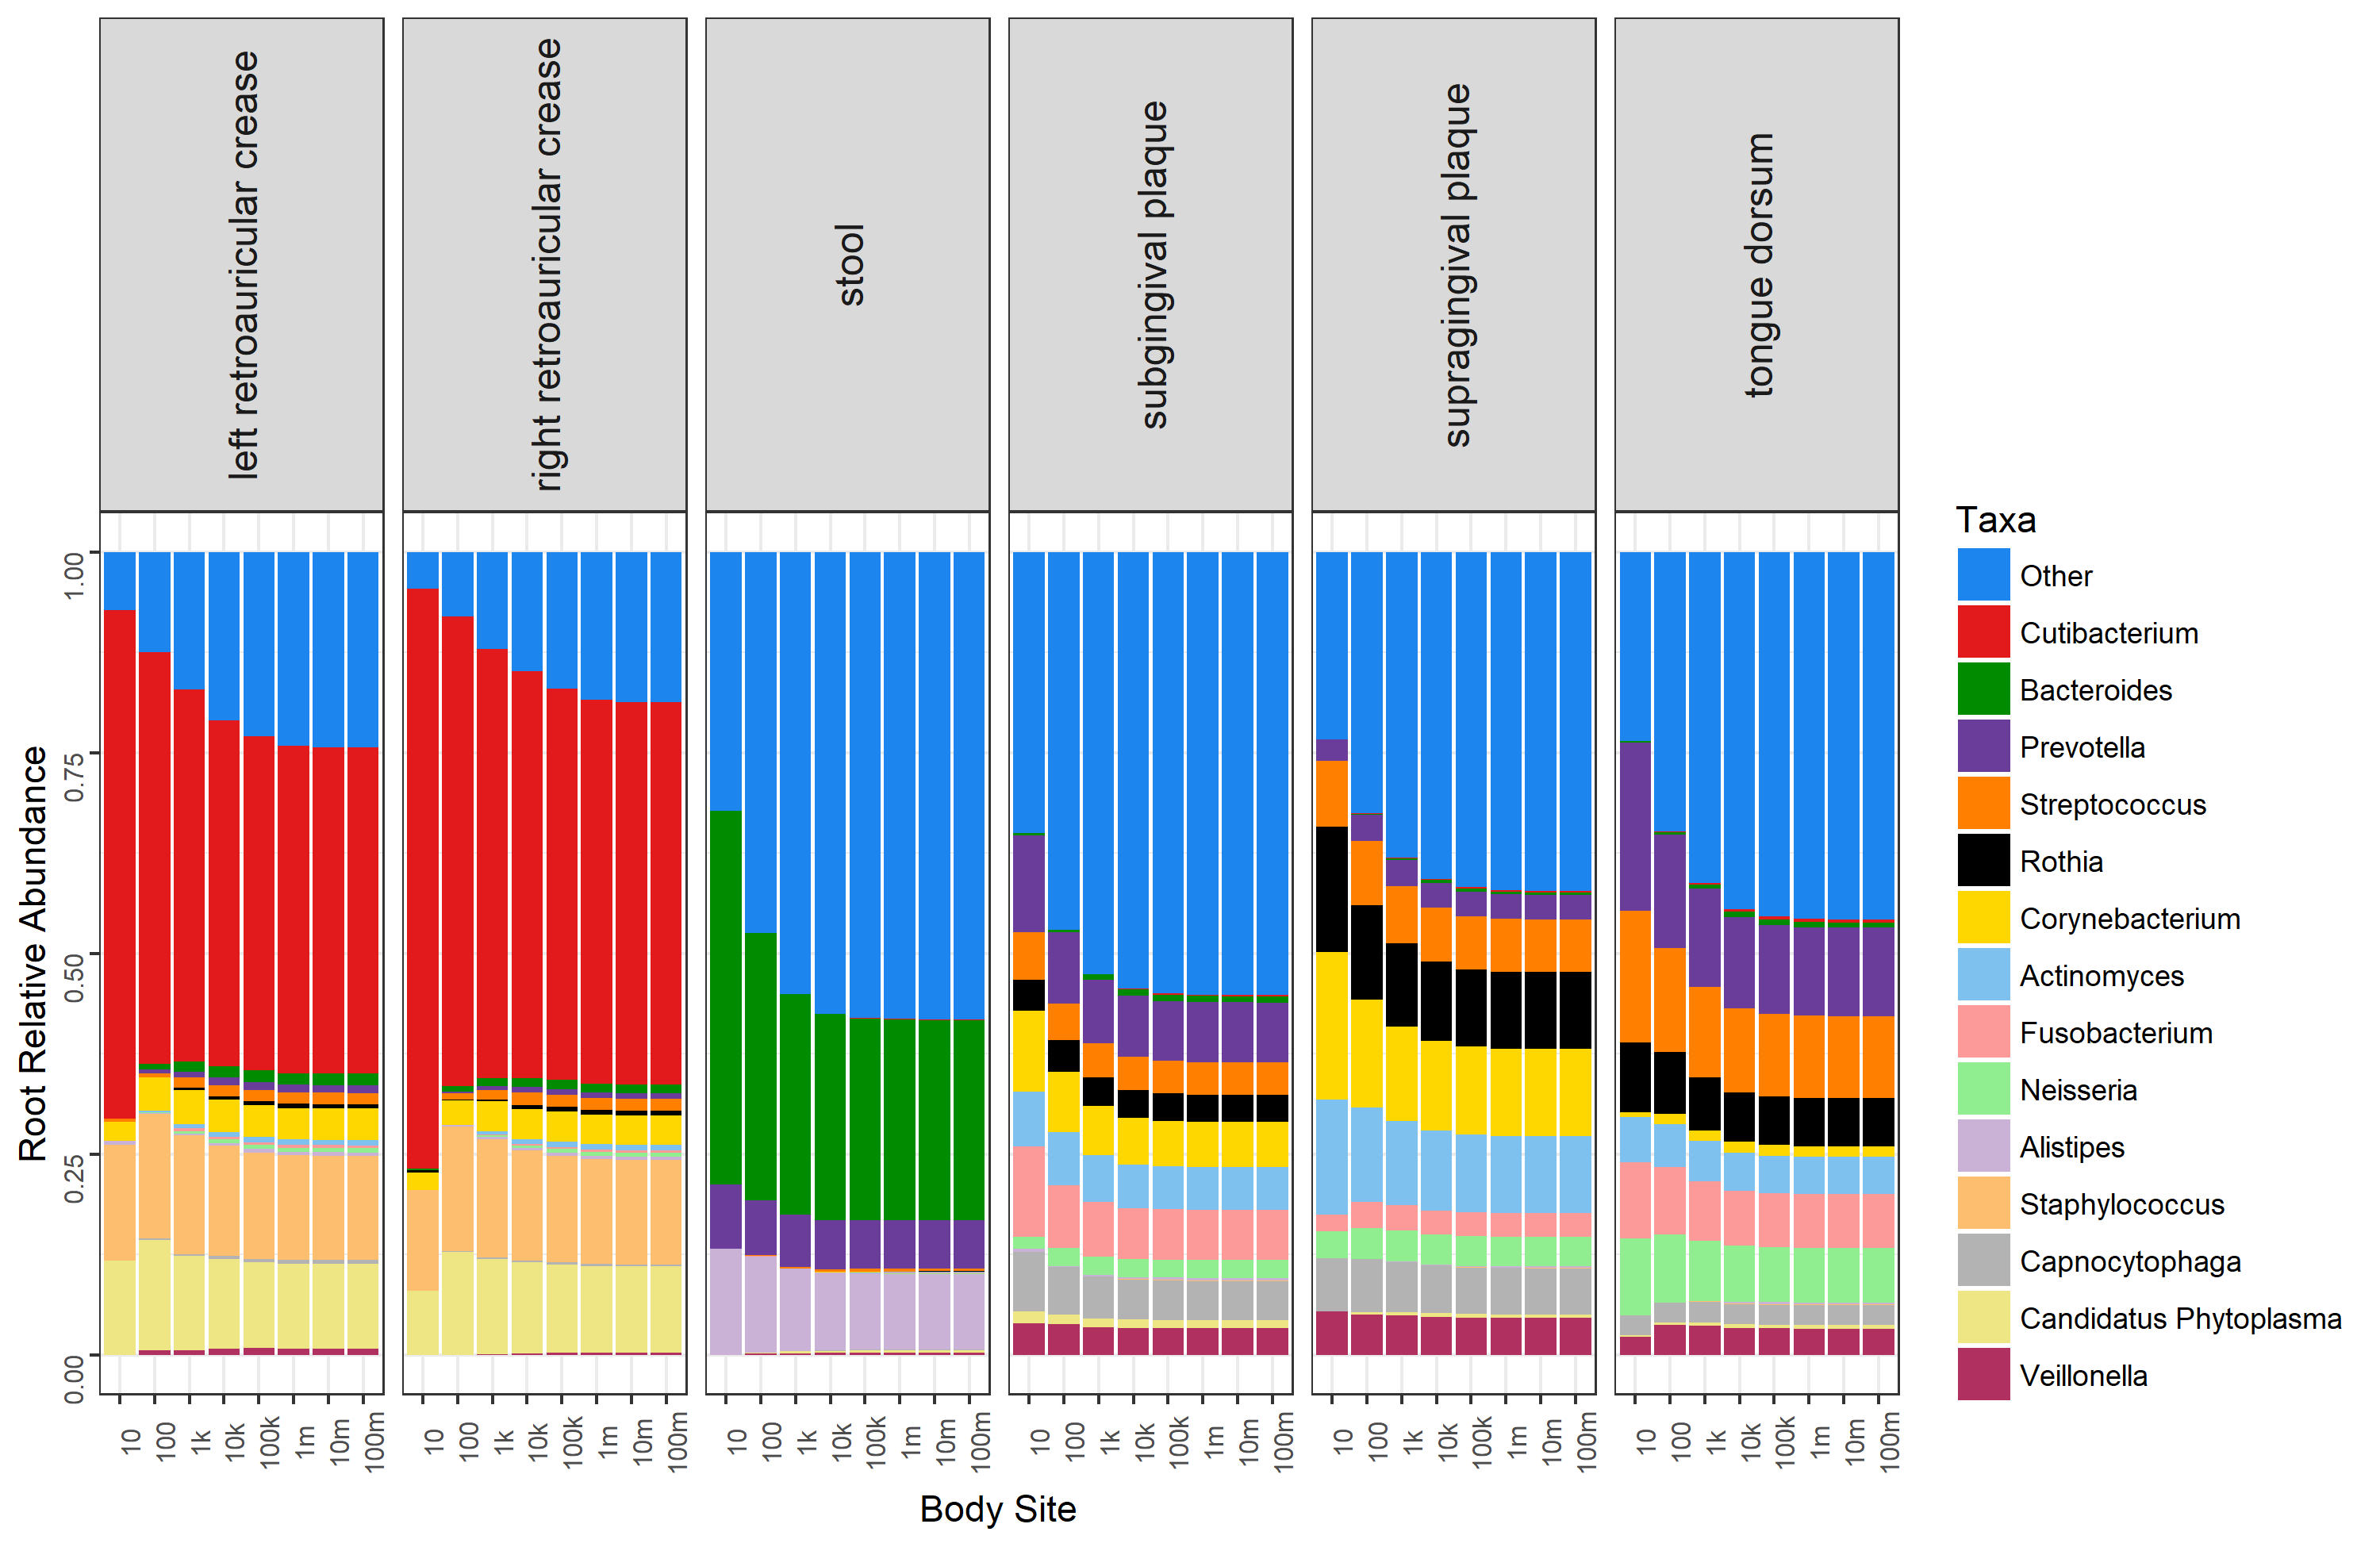
\includegraphics[width=0.99\linewidth]{fig/hmp_taxa.png}
%     \caption{
%         Taxa-summary plots at genus-level (for visualization convenience) stratified by body site by increasing depth. Visually depicted is the transition of the relative abundance vectors to the stabilized full depth relative abundance between a thousand and ten-thousand counts per sample.
%     }
%     \label{fig:hmp_taxa}
% \end{figure}

%%% fig:karlsson2013_f1_combined
\begin{figure}[hbt]
    \centering
    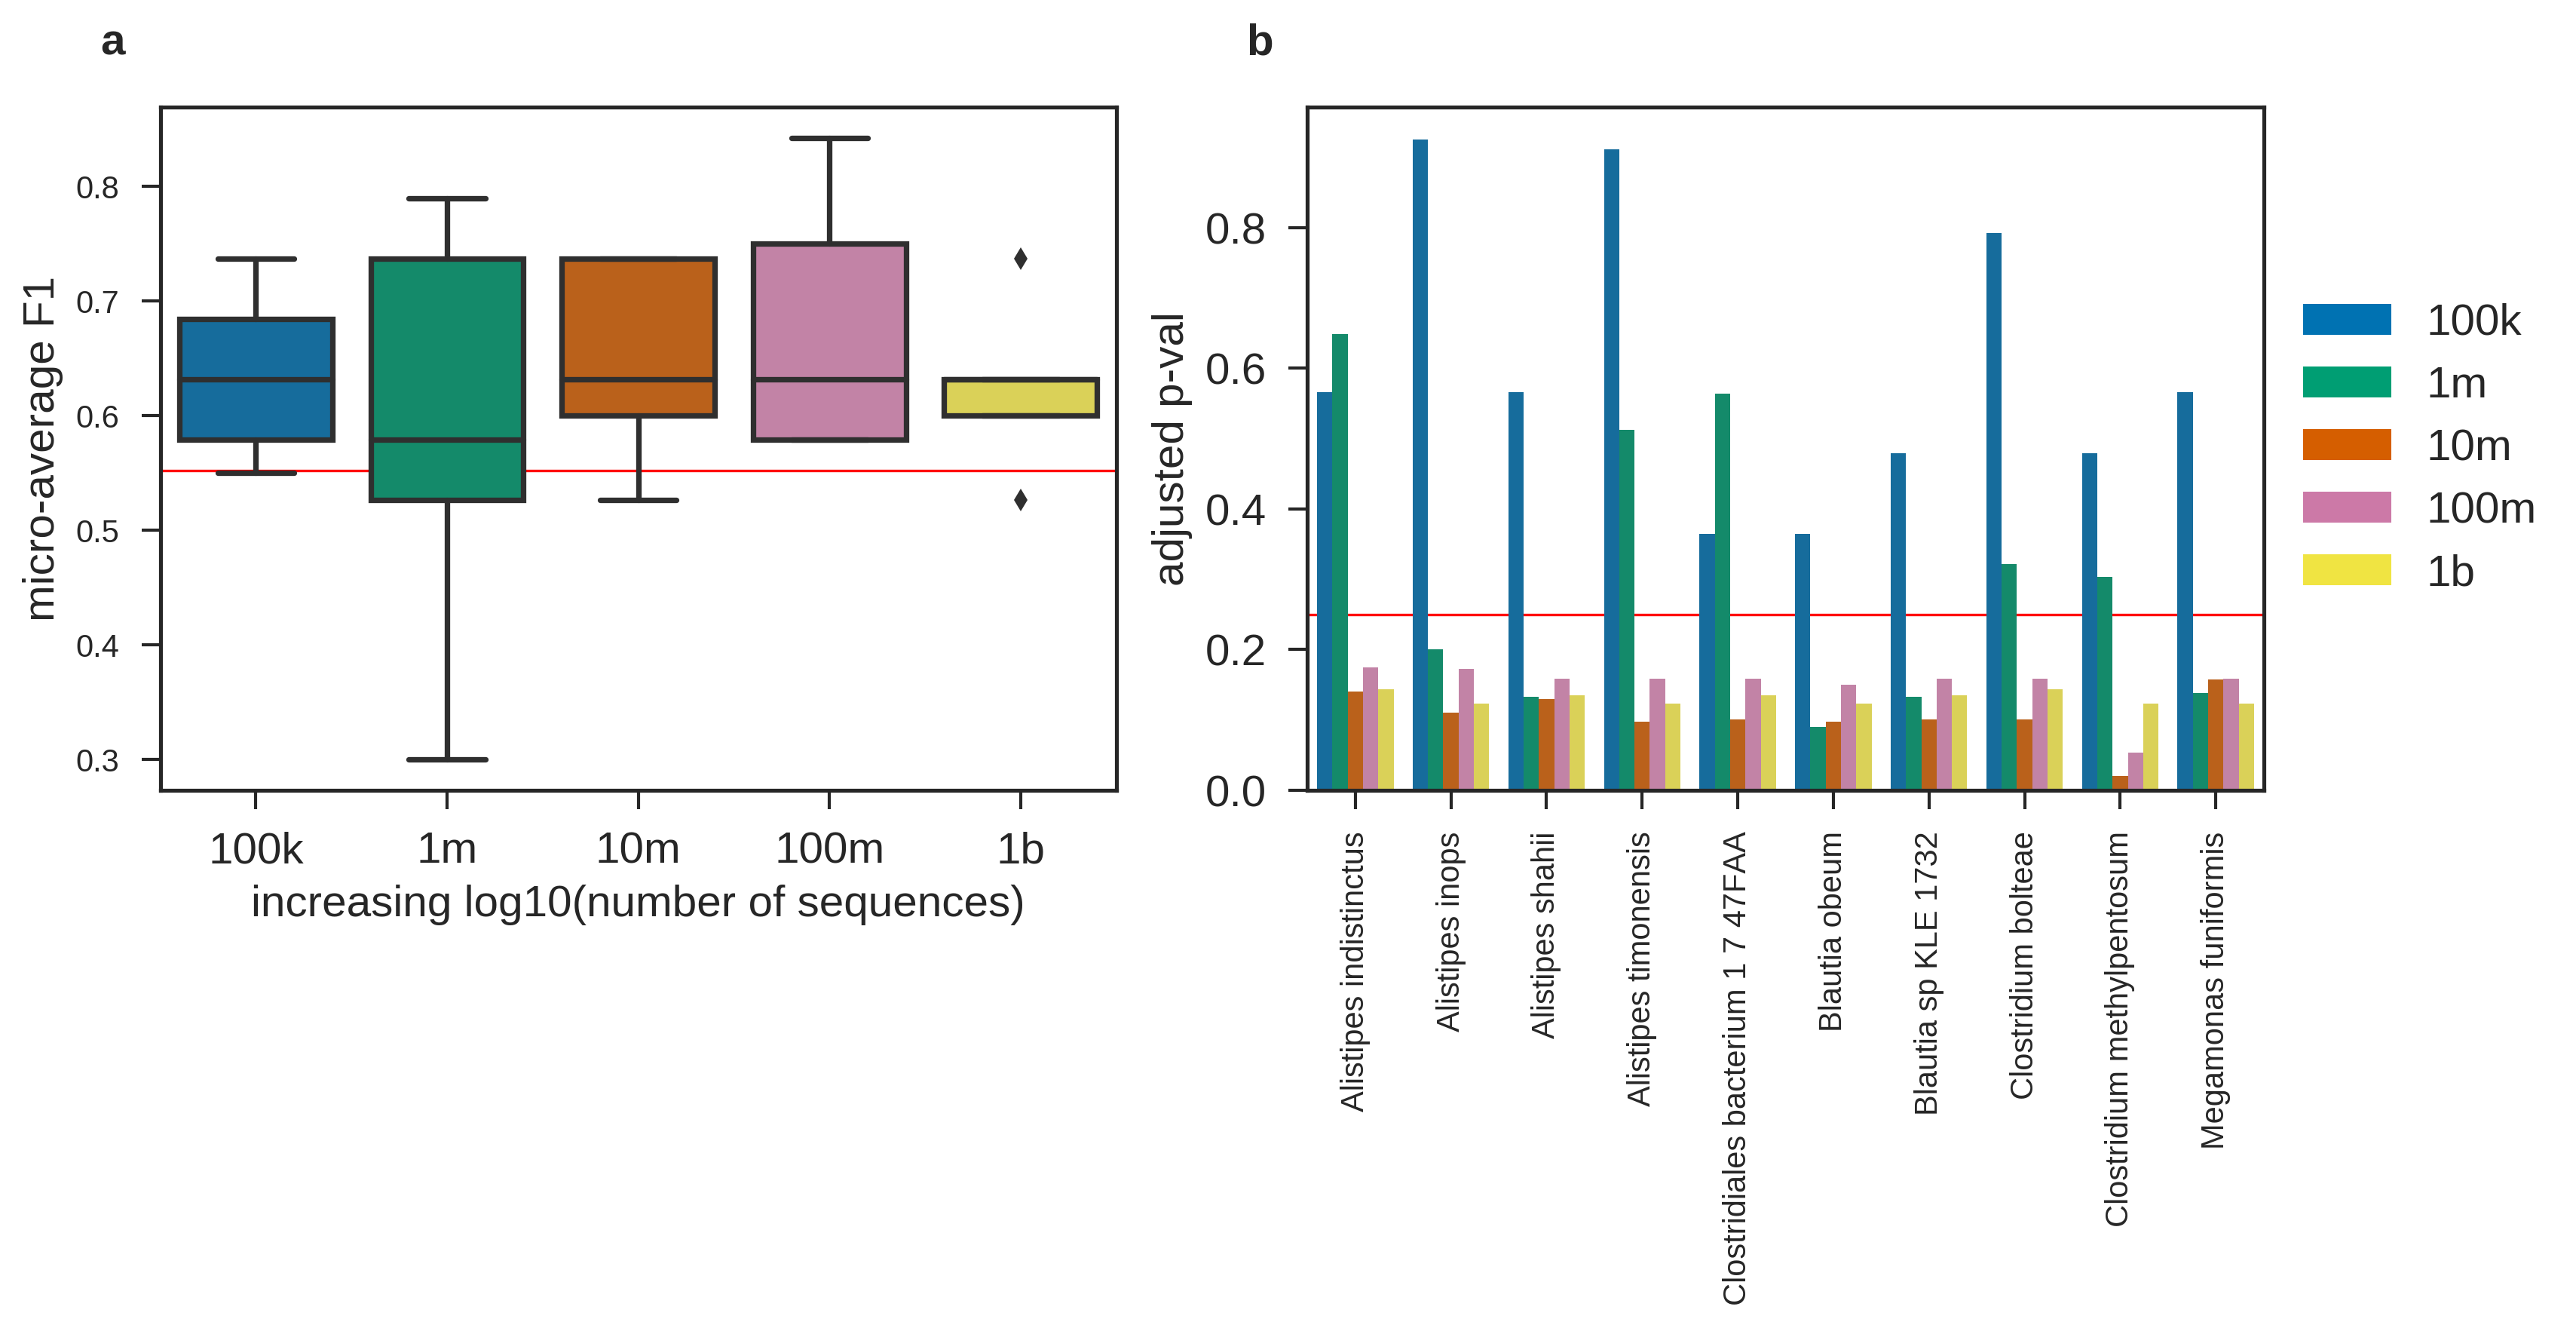
\includegraphics[width=0.8\linewidth]{fig/karlsson2013_f1_combined.png}
    \caption{
        (a) The micro-averaged F1-Score from 10-fold cross-validation on predicting normal glucose tolerance (NGT) versus type-2 diabetes (T2D) on centered log-ration (CLR) multiplicative replacement transformed Karlsson dataset. The classifier used was a Support Vector Machine (SVM) with a linear kernel. The red line is the baseline classifier that predicts majority class (NGT samples = 43, T2D samples = 53). At all subsampled depths, the classifier is able to outperform the baseline classifier verifying the discriminative correlation of microbes with T2D. (b) The Benjamini-Hochberg adjusted Wilcoxon signed-rank p-values for the differentially abundant species between T2D and NGT at varying depths. Displayed are the top ten most differentially abundant species at full depth. The red line is a false-positive rate of 25\%. All species remain significant until a subsampled depth of a thousendth of the original sequences.
    }
    \label{fig:karlsson2013_f1_combined}
\end{figure}

%%% fig:simulations
\begin{figure}[hbt]
    \centering
    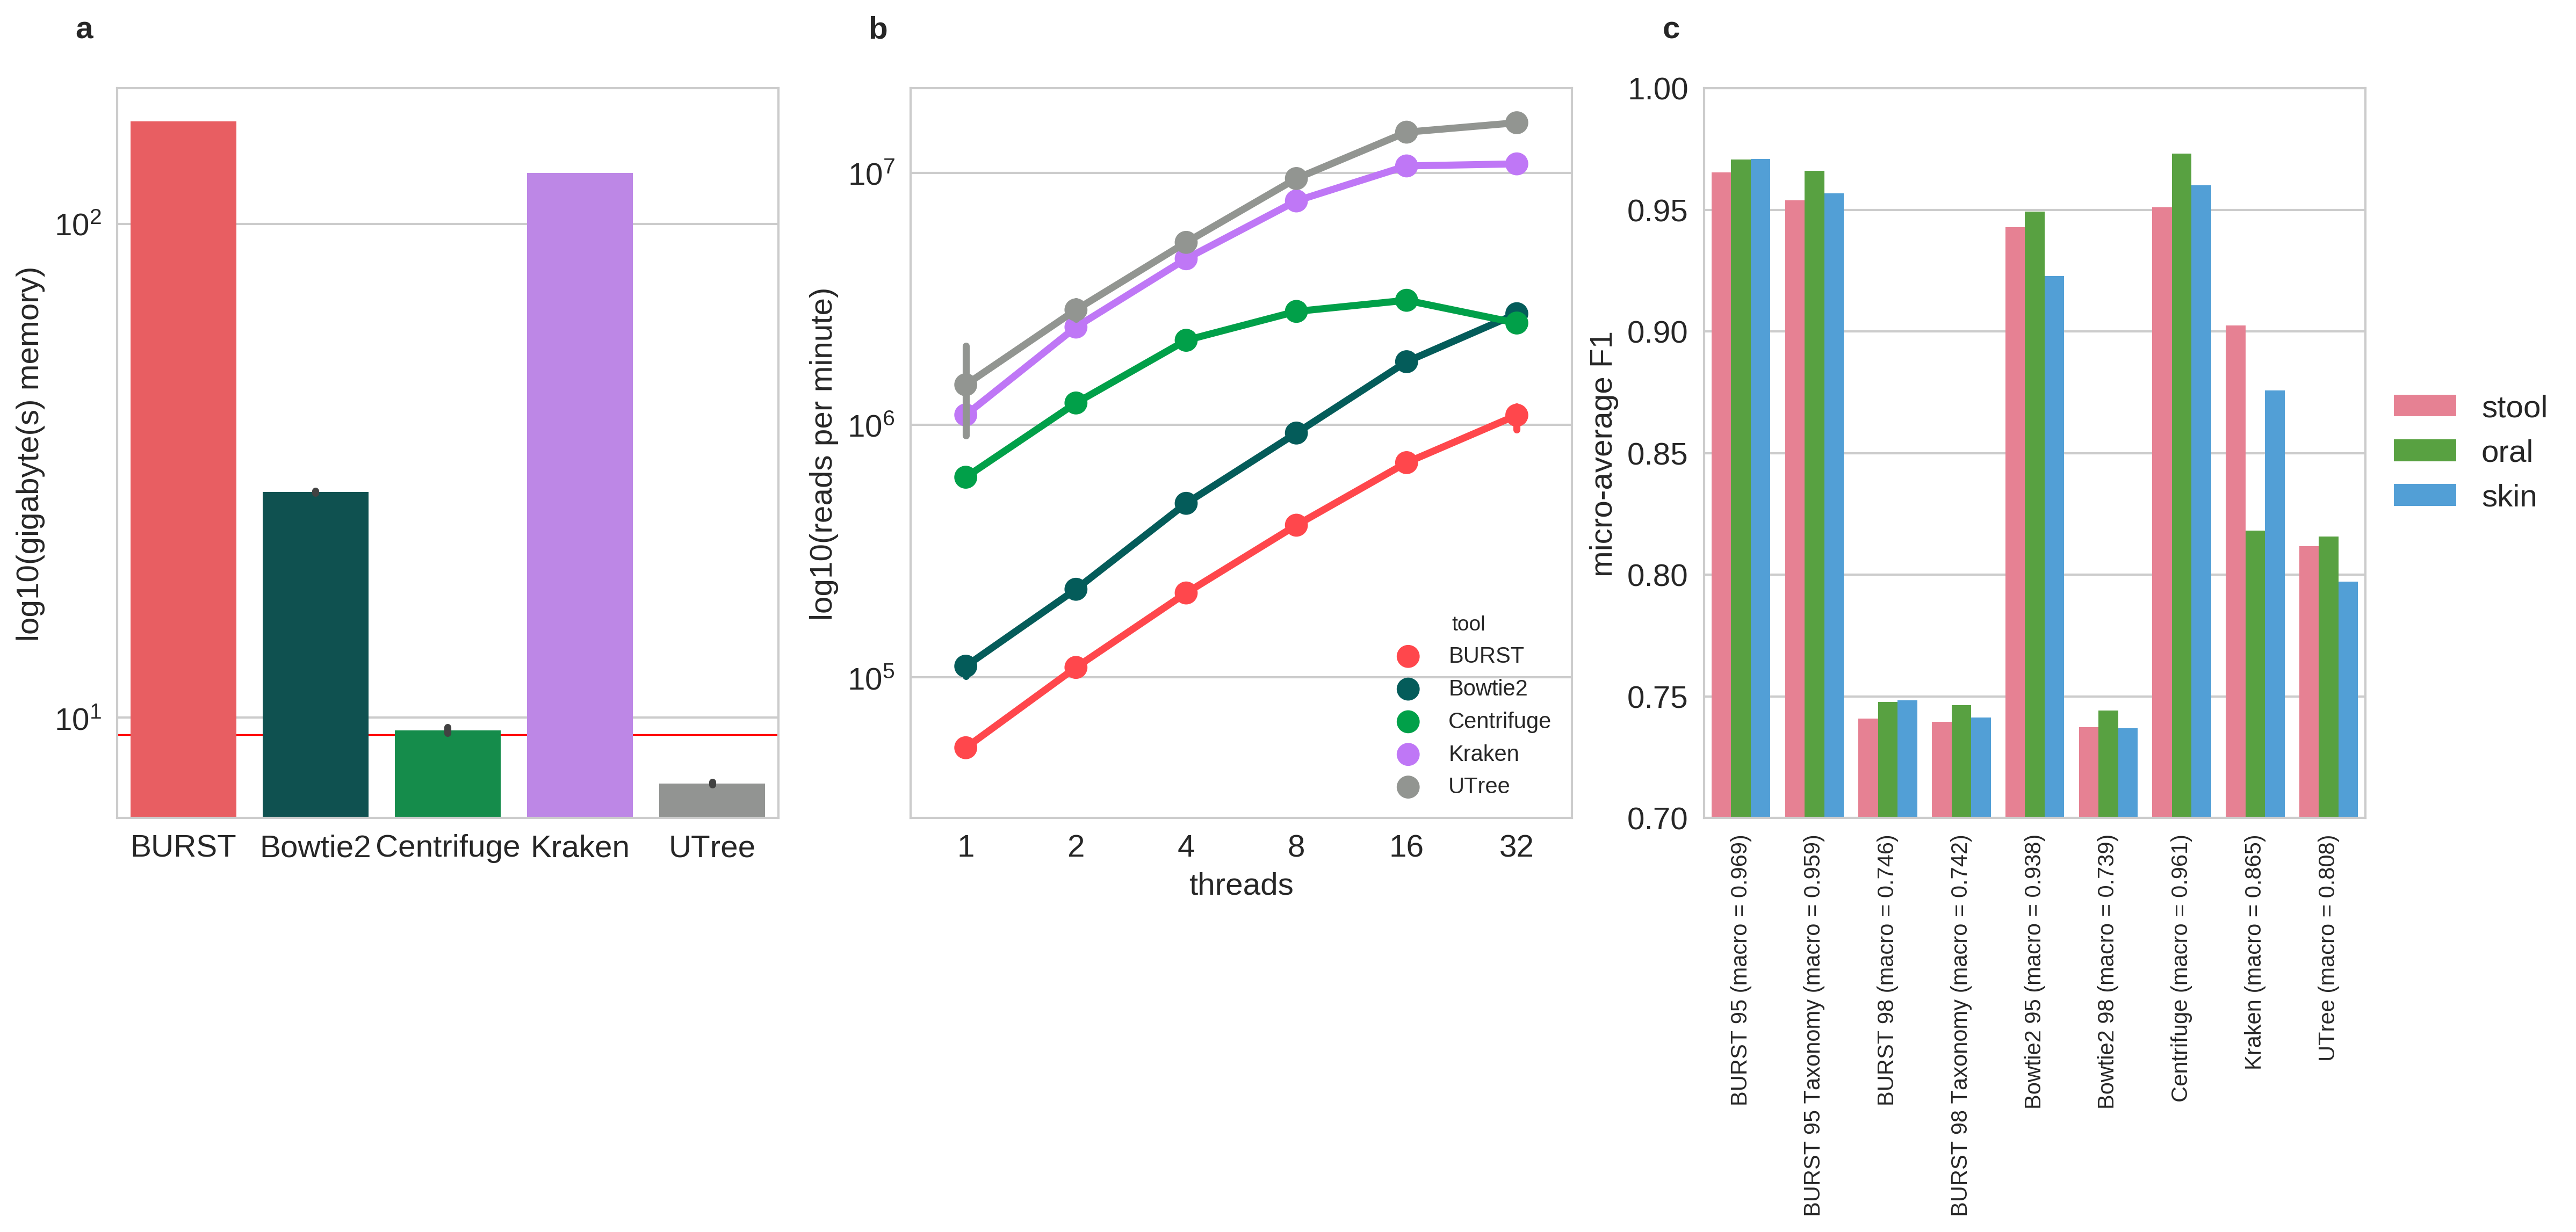
\includegraphics[width=0.8\linewidth]{fig/simulations.png}
    \caption{
        (a) The maximum resident size set (RSS) in Gigabytes of each of the aligners with the Kraken timing dataset. The horizontal red line depicts the size of the original Rep82 database. (b) The scaling and efficiency in reads per minute of each of the aligners across many threads per process. The fastest tools are the alignment free methods Kraken and UTree. Each of the tools scale efficiently across many threads per process. (c) The micro-averaged F1-score of each of the aligners on per read bases on the simulated stool, oral, and skin communities. For the alignment methods, two different thresholds at 95\% and 98\% for alignment identification were set to account for recall bias in highly-divergent reads.
    }
    \label{fig:simulations}
\end{figure}

%%% fig:simulations_js
\begin{figure}[hbt]
    \centering
    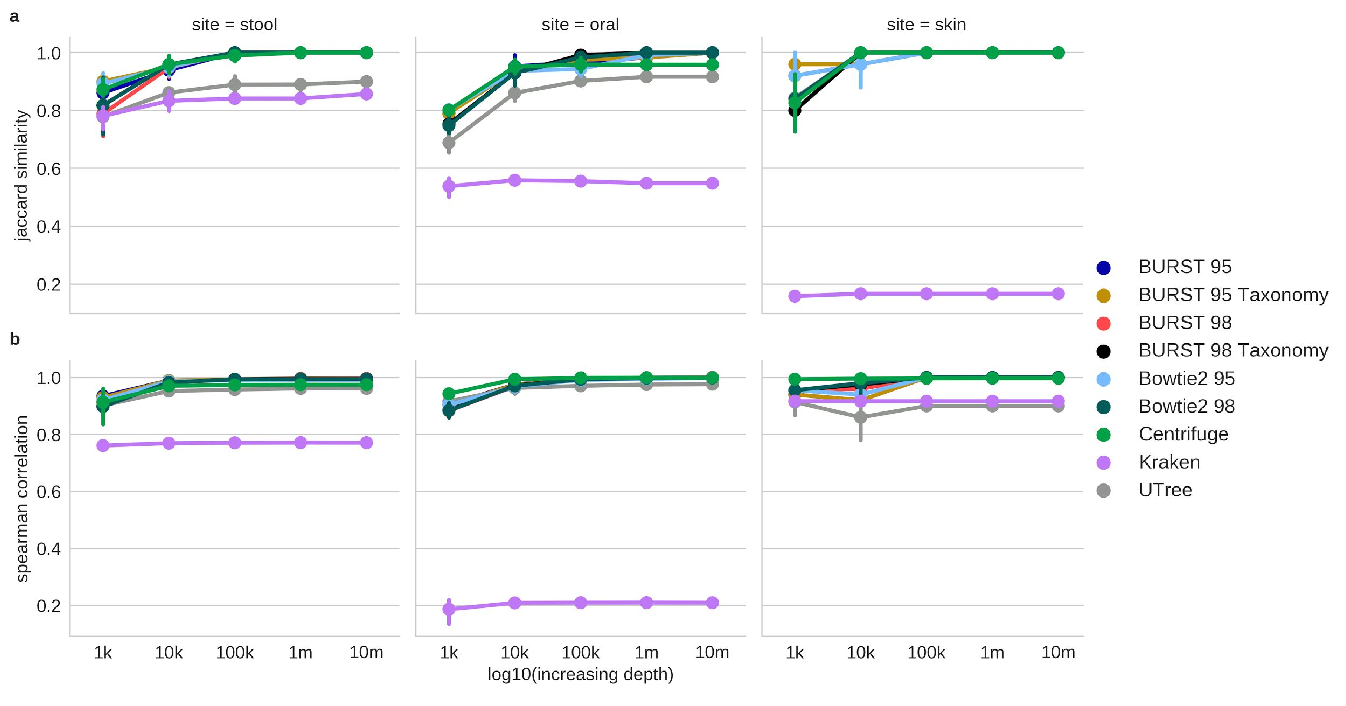
\includegraphics[width=0.8\linewidth]{fig/simulations_js.pdf}
    \caption{
          (a) Rarefaction curves of Jaccard similarity of known species and predicted species for each of the alignment tools on the simulated stool, oral, and skin communities. For most tools, all species are identified between ten-thousand and a hundred thousand reads. (b) The rarefaction curves of Spearman correlation of the tools predicted community with the known community for the simulated dataset. This shows that not only are the correct species identified, but they are also in the correct abundances. 
    }
    \label{fig:simulations_js}
\end{figure}

%%% tab:database_stats
\begin{table}[hbt]
  \centering
  \begin{tabular}{l|r|r}
      \textit{Kingdom} & \textit{Number of Genomes} & \textit{Megabase pairs (Mbp)} \\ \hline
      Archaea & 238 & 627,101.26\\ \hline
      Bacteria & 4,884 & 19,308,087.26\\ \hline
      Plasmid & 614 & 198,476.94\\ \hline
      Viroids & 46 & 15.50\\ \hline
      Viruses & 7,194 & 253,668.36\\ \hline \hline
      \textbf{Total} & \textbf{12,976} & \textbf{20,387,349.32}\\ 
  \end{tabular}
  \caption{
        The number of strains and megabase pairs for each kingdom for all representative Archaea, Bacteria, Plasmid, Viroids and Virus sequences in RefSeq version 82 (Rep82). Each entry in the database is assigned a unique taxonomic string identifier at each level in the taxonomic tree down to strain. An example taxonomic annotation for humans is \code{k\_\_Eukaryota;p\_\_Chordata;c\_\_Mammalia;o\_\_Primates;f\_\_Hominidae;g\_\_Homo;s\_\_Homo\_sapiens;t\_\_}. Each strain is a given a unique entry so that BURST capitalist properly disambiguates reads that hit multiple strains for proper taxonomic profiling and coverage analysis. 
  }
  \label{tab:database_stats}
\end{table}

% Table generated by Excel2LaTeX
%%% tab:discussion
\begin{table}[htbp]
      \centering
      \begin{tabular}{rrll}
      \multicolumn{1}{l}{\textit{Approach}} & \multicolumn{1}{l}{\textit{Examples}} & \textit{Pros} & \textit{Cons} \\
      \midrule
      \midrule
      \multicolumn{1}{l}{\textbf{Last Common Ancestor Alignment}} & \multicolumn{1}{l}{Bowtie2 Taxonomy} & Highest Precision & High RAM \\
            & \multicolumn{1}{l}{BURST Taxonomy} &       & \multicolumn{1}{p{9.5em}}{Slow} \\
            &       &       & No coverage analysis \\
      \midrule
      \multicolumn{1}{l}{\textbf{Exhaustive Alignment}} & \multicolumn{1}{l}{BURST Capitalist} & Highest F1 Accuracy & High RAM \\
            &       & Highest Recall & Slow \\
      \midrule
      \multicolumn{1}{l}{\textbf{Marker Gene}$^\dagger$} & \multicolumn{1}{l}{Metaphlan} & Low RAM & Sparse Database \\
            &       & Fast  &  \\
      \midrule
      \multicolumn{1}{l}{\textbf{Exact K-mers}} &       & Fastest & No coverage analysis \\
            &       &       & Sensitive to indels \\
      \cdashlinelr{2-4}
            & \multicolumn{1}{l}{Kraken} &       & High RAM \\
            &       &       & Large Database \\
      \cdashlinelr{2-4}
            & \multicolumn{1}{l}{Utree} & Lowest RAM &  \\
            &       & Smallest Database &  \\
      \midrule
      \multicolumn{1}{l}{\textbf{Longest Common Substring}} & \multicolumn{1}{l}{Centrifuge} & Fast  & No coverage analysis \\
            &       & Low RAM & Sensitive to indels \\
      \bottomrule
      \multicolumn{4}{l}{$^\dagger$\footnotesize{ Marker gene taxonomic profilers were not evaluated in this study due to complexity of creating a database and low alignment rates.}}
      \end{tabular}%
      \caption{
            Summarization of the many tools tested in this paper for shallow-shotgun sequencing. While this list is not comprehensive, we recommend using any tools in the approaches listed as legitimate options for analysis of shallow-shotgun data except for a marker gene$^\dagger$ approach. From the tools surveyed, we found that BURST capitalist returns the most accurate results if properly tuned at the cost of high RAM usage and compute time. If computer resources is a concern, we recommend using either UTree on a computer with over 8GB RAM or Centrifuge on a computer with over 16GB RAM.
      }
      \label{tab:discussion}
\end{table}


\end{document}
